\documentclass[journal]{IEEEtran}

\usepackage{amsmath,amsfonts,amssymb}
\usepackage{array}
\usepackage[caption=false,font=normalsize,labelfont=sf,textfont=sf]{subfig}
\usepackage{textcomp}
\usepackage{stfloats}
\usepackage{url}
\usepackage{graphicx}
\usepackage{booktabs}
\usepackage[table]{xcolor}
\usepackage{cite}
\usepackage{tikz}
\usetikzlibrary{positioning,arrows.meta}
\usepackage{pgfplots}
\pgfplotsset{compat=1.18}
\usepackage{circuitikz}
\usepackage{jabbrv}

\hyphenation{op-tical net-works semi-conduc-tor IEEE-Xplore}

% Compiles even when a draft figure file is not yet available.
\newcommand{\figplaceholder}[3]{%
\fbox{\parbox[c][#2][c]{#1}{\centering\footnotesize #3}}%
}

\begin{document}

\title{Stacked Polyphase Bridge Converters for High-Voltage Electric
Traction Drives: A Review of Topology, Modulation, Control,
Semiconductor Scaling, and Research Challenges}

\author{Enes~Ayaz,~\IEEEmembership{Student Member,~IEEE},
Shahriar~Sarmast~Ghahfarokhi,~\IEEEmembership{Student Member,~IEEE},
Staffan~Norrga,~\IEEEmembership{Member,~IEEE},
Hans-Peter~Nee,~\IEEEmembership{Fellow,~IEEE}%
\thanks{(Corresponding author: Enes Ayaz.)}%
\thanks{E. Ayaz, S. Sarmast Ghahfarokhi, S. Norrga, and H.-P. Nee
are with the Division of Electric Power and Energy Systems,
KTH Royal Institute of Technology, SE-100~44 Stockholm, Sweden
(e-mail: enesa@kth.se).}%
}

\markboth{}%
{Ayaz \MakeLowercase{\textit{et al.}}: Stacked Polyphase Bridge Converters}

\maketitle

\begin{abstract}
Higher dc-link voltage is increasingly attractive in electric traction, but it raises semiconductor blocking-voltage, switching-transient, insulation, and electromagnetic-compatibility demands. The stacked polyphase bridge (SPB) addresses the semiconductor-voltage problem by connecting three-phase two-level bridges in series on the dc side, each supplying an electrically separated winding group — a voltage-partitioning approach that accesses lower-voltage semiconductor classes and supports modular converter–machine integration, at the cost of added winding, dc-link, sensing, gate-drive, and insulation-coordination overhead. Although SPB has been studied for over a decade, the literature remains scattered across topology, modulation, common-mode voltage, dc-link balancing, multiphase-machine design, semiconductor technology, and fault-tolerant control, without a common system-boundary evaluation. This review consolidates SPB's evolution, operating principle, and machine-integration options (aligned, spatially shifted, and physically segmented winding groups); derives the double Fourier series basis for its interleaved-carrier dc-link current ripple; quantifies common-mode-voltage cancellation, switching-delay-induced residual spikes, and the resulting bearing current; analyzes dc-link voltage-balancing stability from the exact nonlinear cell model across centralized, common-duty-ratio, and distributed control; and examines semiconductor scaling and post-fault operation using reported experimental fault data. A cell-count-to-voltage-class mapping with a commercial-device screening approach is developed for a 1200-V dc link, showing that lower device-voltage classes can yield nonlinear semiconductor-level gains while converter and machine hardware scale roughly with cell count, so the preferred cell count is mission-dependent rather than fixed. SPB should therefore be assessed as a modular converter–machine architecture whose competitiveness depends on whether voltage partitioning yields a system-level benefit sufficient to justify its added integration and control complexity.
\end{abstract}

\begin{IEEEkeywords}
Electric vehicles, integrated motor drives, modular converters,
multiphase machines, stacked polyphase bridge (SPB) converters.
\end{IEEEkeywords}

% ============================================================================
\section{Introduction}
\label{sec:introduction}
% ============================================================================

Electrification is pushing traction-drive propulsion and fast-charging
power toward several hundred kilowatts, while system-level performance
requirements continue to rise \cite{EVTractionReview2023}. Increasing
the dc-link voltage has emerged as a primary design lever for meeting
both demands. On the propulsion side, a higher dc-link voltage
improves efficiency and power density \cite{DriveCodesign800V2023}. On
the battery and charging side, it reduces the current required for a
given power level, lowering cable conduction loss and conductor
cross-section while enabling higher charging power under a given
current limit \cite{Post800V2026}.

This trend, however, is not without consequence at the converter
level. A higher dc-link voltage also brings more severe
insulation-coordination and electromagnetic-compatibility (EMC)
demands, together with added thermal and reliability stress on the
power stage \cite{DriveCodesign800V2023,Post800V2026}.
Fig.~\ref{fig:intro_hv_motivation} summarizes this qualitative
tradeoff between a conventional low-voltage and a higher-voltage
traction architecture. Raising the dc-link voltage therefore does not
amount to a simple rescaling of an existing inverter design; it
reshapes the architecture-level design space of the complete electric
drive.


\begin{figure}[!t]
\centering
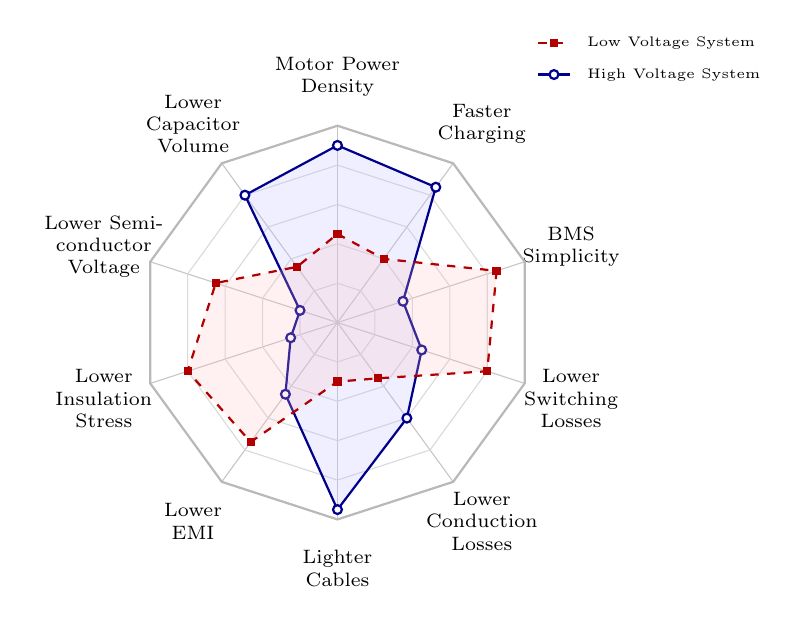
\begin{tikzpicture}[font=\scriptsize,>=latex]
\def\R{2.5}
% illustrative, qualitative per-axis extent (not measured/simulated data)
% axis order (i=0..9, angle=90-i*36): Motor Power Density, Faster
% Charging, BMS Simplicity, Lower Switching Losses, Lower Conduction
% Losses, Lighter Cables, Lower EMI, Lower Insulation Stress, Lower
% Semiconductor Voltage, Lower Capacitor Volume
\foreach \i/\lab in {0/{Motor Power\\Density},1/{Faster\\Charging},
  2/{BMS\\Simplicity},3/{Lower Switching\\Losses},
  4/{Lower Conduction\\Losses},5/{Lighter\\Cables},6/{Lower\\EMI},
  7/{Lower Insulation\\Stress},8/{Lower Semiconductor\\Voltage},
  9/{Lower Capacitor\\Volume}}{
  \pgfmathsetmacro{\ang}{90-\i*36}
  \draw[gray!45,thin] (0,0) -- (\ang:\R);
  \node[align=center,text width=17mm] at (\ang:\R+0.62) {\lab};
}
\foreach \rr in {0.5,1.0,1.5,2.0,2.5}{
  \draw[gray!30,thin] (90:\rr) \foreach \i in {1,...,9}{
    -- (90-\i*36:\rr)
  } -- cycle;
}
\draw[gray!55,thick] (90:\R) \foreach \i in {1,...,9}{
  -- (90-\i*36:\R)
} -- cycle;
% High-voltage system (blue, solid, open circle markers)
\draw[blue!55!black,thick,fill=blue!25,fill opacity=0.25]
  (90:0.90*\R) -- (54:0.85*\R) -- (18:0.35*\R) -- (-18:0.45*\R)
  -- (-54:0.60*\R) -- (-90:0.95*\R) -- (-126:0.45*\R)
  -- (-162:0.25*\R) -- (162:0.20*\R) -- (126:0.80*\R) -- cycle;
\foreach \ang/\v in {90/0.90,54/0.85,18/0.35,-18/0.45,-54/0.60,
  -90/0.95,-126/0.45,-162/0.25,162/0.20,126/0.80}{
  \node[draw=blue!55!black,fill=white,circle,thick,
    minimum size=3.2pt,inner sep=0pt] at (\ang:\v*\R) {};
}
% Low-voltage system (red, dashed, filled square markers)
\draw[red!70!black,thick,dashed,fill=red!25,fill opacity=0.22]
  (90:0.45*\R) -- (54:0.40*\R) -- (18:0.85*\R) -- (-18:0.80*\R)
  -- (-54:0.35*\R) -- (-90:0.30*\R) -- (-126:0.75*\R)
  -- (-162:0.80*\R) -- (162:0.65*\R) -- (126:0.35*\R) -- cycle;
\foreach \ang/\v in {90/0.45,54/0.40,18/0.85,-18/0.80,-54/0.35,
  -90/0.30,-126/0.75,-162/0.80,162/0.65,126/0.35}{
  \node[draw=red!70!black,fill=red!70!black,
    minimum width=2.6pt,minimum height=2.6pt,inner sep=0pt]
    at (\ang:\v*\R) {};
}
% Legend, upper right, line+marker style
\draw[red!70!black,thick,dashed] (2.55,3.55) -- (2.95,3.55);
\node[draw=red!70!black,fill=red!70!black,minimum width=2.6pt,
  minimum height=2.6pt,inner sep=0pt] at (2.75,3.55) {};
\node[anchor=west,font=\tiny] at (3.05,3.55) {Low Voltage System};
\draw[blue!55!black,thick] (2.55,3.15) -- (2.95,3.15);
\node[draw=blue!55!black,fill=white,circle,thick,minimum size=3.2pt,
  inner sep=0pt] at (2.75,3.15) {};
\node[anchor=west,font=\tiny] at (3.05,3.15) {High Voltage System};
\end{tikzpicture}
\caption{Conceptual illustration of the qualitative system-level
tradeoffs between a low-voltage and a high-voltage traction
architecture.}
\label{fig:intro_hv_motivation}
\end{figure}

\subsection{Literature and Industry Trends Toward Higher DC-Link Voltage}

The trend motivated above is not merely conceptual: it is already
established in academic prototypes, industrial inverter platforms, and
production vehicles, as summarized in
Table~\ref{tab:intro_voltage_power}. Reported academic demonstrators
range from 400-V to 800-V and 1.2-kV converters, with still higher
levels investigated for high-power passenger and heavy-duty
applications \cite{Post800V2026}, while industrial platforms
increasingly target 800-V operation as a baseline and production
vehicles show a comparable shift from established 400-V architectures
to a growing number of 800-V and higher-voltage platforms
\cite{Aghabali2021TTE800V,Mousavi2025ICTEM800V}. This industry-wide
direction, rather than an isolated research interest, motivates the
semiconductor-level analysis that follows since the rising dc-link voltages
translate directly into a semiconductor-level bottleneck.

\begin{table*}[!t]
\caption{Representative voltage and power levels in published
traction-inverter studies, industrial and reference platforms, and
production battery-electric vehicles. }
\label{tab:intro_voltage_power}
\centering
\footnotesize
\renewcommand{\arraystretch}{1.18}
\setlength{\tabcolsep}{6pt}

\begin{tabular}{
p{0.25\textwidth}
p{0.32\textwidth}
p{0.36\textwidth}}
\hline

\multicolumn{1}{l}{\textbf{Published studies / demonstrators}} &
\multicolumn{1}{l}{\textbf{Industrial / reference platforms}} &
\multicolumn{1}{l}{\textbf{Production vehicles}} \\

\hline

\textbf{Bertelshofer et al.}:
400~V, 150~kW
\cite{Bertelshofer2019SiC150kW}
&
\textbf{Bosch Gen.~4}:400/800~V, 250/350~kW
\cite{BoschInverterGen4}
&
\textbf{BMW i4 M50}:
400~V, 400~kW
\cite{BMWi4M50Specifications}
\\

\textbf{Taha et al.}:
800~V, 100~kW
\cite{Taha2024SixPhase100kW}
&
\textbf{Wolfspeed reference design}:
800~V, 300~kW
\cite{TIWolfspeed300kW}
&
\textbf{Hyundai IONIQ 5 N}:
800~V, 478~kW
\cite{HyundaiIoniq5N2026}
\\

\textbf{Al-Hmoud et al.}:
1~kV, 200~kW
\cite{AlHmoud2023Traction}
&
\textbf{Infineon eCAV platform}:
800~V, 250~kW
\cite{InfineonCAV250kW}
&
\textbf{Volvo EX90 Performance}:
800~V, 500~kW
\cite{VolvoEX90Specifications2026}
\\

\textbf{Wang et al.}:
1.2~kV, 100~kW
\cite{Wang2021ANPC1200V}
&
\textbf{AVL PI850e}:
800~V, 250~kW
\cite{AVLPI850e}
&
\textbf{Porsche Taycan Turbo S}:
800~V, 700~kW
\cite{PorscheTaycanTurboS2026}
\\

\textbf{Ayaz et al.}:
1.2~kV, 250~kW
\cite{TwoLevel_Enes}
&
\textbf{Punch IV5}:
800~V, 600~kW
\cite{PunchIV5}
&
\textbf{Lucid Air Dream Performance}:
900~V, 828~kW
\cite{LucidAirDreamPerformance}
\\

\hline
\end{tabular}
\end{table*}

\subsection{Semiconductor Blocking-Voltage Tradeoff}

\label{sec:semiconductor_limitations}

In a conventional two-level voltage-source inverter, each active
switch must block a voltage directly tied to the complete dc-link
voltage. In unipolar power devices, a higher blocking-voltage rating
imposes a fundamental tradeoff against both specific on-state
resistance and switching performance, commonly captured by the figure
of merit, as shown in Fig.~\ref{fig:intro_ronsp_trend}
\cite{Millan2014WBGSurvey,SpecificResistance}. Therefore, a lower-voltage device
consistently achieves a higher FOM than a higher-voltage device of the
same material.

\begin{figure}[!t]
\centering
\resizebox{\columnwidth}{!}{%
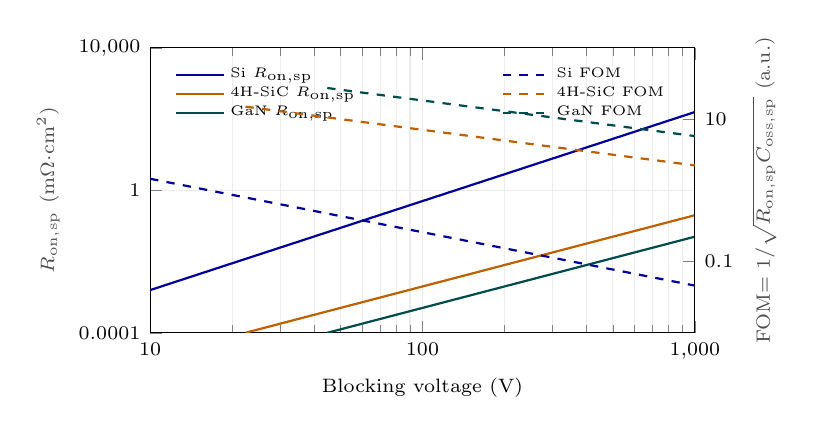
\begin{tikzpicture}
\begin{axis}[
    width=8.5cm,
    height=52mm,
    font=\scriptsize,
    xlabel={Blocking voltage (V)},
    ylabel={$R_{\mathrm{on,sp}}$ (m$\Omega\cdot$cm$^2$)},
    xmode=log, ymode=log,
    log ticks with fixed point,
    xmin=10,xmax=1000,
    ymin=1e-4,ymax=1e4,
    tick label style={font=\scriptsize},
    xlabel style={font=\scriptsize},
    ylabel style={font=\scriptsize,black!70},
    axis y line*=left,
    grid=both,
    grid style={gray!15},
    legend style={font=\tiny,draw=none,fill=none,
      at={(0.03,0.97)},anchor=north west,row sep=-2pt},
    legend cell align=left,
]
\addplot[blue!60!black,thick,solid,domain=10:1000,samples=60] {5e-6*x^2.5};
\addlegendentry{Si $R_{\mathrm{on,sp}}$}
\addplot[orange!75!black,thick,solid,domain=22.4:1000,samples=60] {2e-7*x^2};
\addlegendentry{4H-SiC $R_{\mathrm{on,sp}}$}
\addplot[teal!60!black,thick,solid,domain=44.7:1000,samples=60] {5e-8*x^2};
\addlegendentry{GaN $R_{\mathrm{on,sp}}$}
\end{axis}
\begin{axis}[
    width=8.5cm,
    height=52mm,
    font=\scriptsize,
    xmode=log, ymode=log,
    log ticks with fixed point,
    xmin=10,xmax=1000,
    ymin=1e-2,ymax=1e2,
    axis y line*=right,
    axis x line=none,
    ylabel={FOM$=1/\sqrt{R_{\mathrm{on,sp}}C_{\mathrm{oss,sp}}}$ (a.u.)},
    ylabel style={font=\scriptsize,black!70},
    tick label style={font=\scriptsize},
    legend style={font=\tiny,draw=none,fill=none,
      at={(0.97,0.97)},anchor=north east,row sep=-2pt},
    legend cell align=left,
]
\addplot[blue!60!black,thick,dashed,domain=10:1000,samples=60] {8.17*x^(-0.75)};
\addlegendentry{Si FOM}
\addplot[orange!75!black,thick,dashed,domain=22.4:1000,samples=60] {70.7*x^(-0.5)};
\addlegendentry{4H-SiC FOM}
\addplot[teal!60!black,thick,dashed,domain=44.7:1000,samples=60] {182.6*x^(-0.5)};
\addlegendentry{GaN FOM}
\end{axis}
\end{tikzpicture}}
    \caption{Ideal one-dimensional unipolar specific on-state
    resistance $R_{\mathrm{on,sp}}$ (left axis, solid) and the
    resulting high-frequency figure of merit
    $\mathrm{FOM}=1/\sqrt{R_{\mathrm{on,sp}}C_{\mathrm{oss,sp}}}$
    (right axis, dashed, arbitrary units) versus blocking voltage for
    Si, 4H-SiC, and GaN.}
    \label{fig:intro_ronsp_trend}
\end{figure}

Wide-bandgap (WBG) semiconductors shift this FOM favorably: SiC
metal-oxide-semiconductor field-effect transistors (MOSFETs) now
dominate high-voltage automotive drives, while GaN is particularly
attractive at lower voltage owing to its fast switching behavior and
superior FOM \cite{WideReview2018,WBGTractionReview2025,GaNComparison,
Millan2014WBGSurvey}. 
Yet switching material does not remove the
underlying coupling between dc-link voltage and device voltage class:
irrespective of technology, a higher dc-link voltage still forces a
higher-voltage, higher-$R_{\mathrm{on,sp}}$ device and higher swithcing losses. 
Converter architectures that partition the dc-link voltage among multiple
switching units, so each device blocks only a fraction of the total
voltage, therefore become increasingly relevant as system voltage
rises.

\subsection{Multilevel Converters and Their Limitations}

Multilevel converters constitute an established solution to this
voltage-partitioning problem.
NPC, T-type, flying-capacitor, and cascaded architectures all distribute
the dc-link voltage among
additional semiconductor positions or capacitor-voltage levels,
reducing individual device voltage stress
\cite{Poorfakhraei2021MultilevelReview,T_type_SiC,
FlyingCap_Optimized3D,CascadedHBridge_control}.

This voltage partitioning, however, comes at the cost of additional
semiconductor devices, passive components, and gate drivers -- each an
additional potential failure point -- without, by itself, yielding a
modular converter--machine system: because the added semiconductor
positions continue to feed a single, electrically common three-phase
winding set, a fault at one position cannot generally be isolated and
bypassed without disabling the drive.
 Fault tolerance, power
redistribution, and post-fault reconfiguration can be implemented in
conventional multilevel drives, but typically require additional
redundancy, dedicated isolation paths, and specialized control layered
on top of the base topology rather than following from it. A larger
semiconductor count therefore does not yield a commensurate increase
in fault tolerance, motivating an alternative form of voltage
partitioning.

\subsection{Stacked Polyphase Bridge}
\label{sec:spb_modularity}

Unlike other multilevel converters, which distribute the dc-link
voltage among additional semiconductor positions within a single
converter, the stacked polyphase bridge (SPB) distributes the
high-voltage conversion function among $N$ repeated converter units.
Each unit is a conventional three-phase two-level bridge connected in
series on the dc side, supplying its own electrically separated
three-phase winding group of the same machine, as illustrated in
Fig.~\ref{fig:spb_architecture}.

Under balanced operation, each cell's local dc-link voltage
$V_{\mathrm{dc},k}\approx V_{\mathrm{dc}}/N$, so the semiconductor
voltage rating can be selected on the local cell voltage rather than
the complete traction dc-link voltage -- addressing the semiconductor
bottleneck much as multilevel converters do. Because each cell also
drives its own separated winding group, however, SPB additionally has
an inherently modular structure that multilevel converters lack: a
faulted cell can, in principle, be isolated and bypassed while the
remaining cells continue to drive the machine at reduced power. It is
this combination of semiconductor voltage reduction and
converter--machine modularity that distinguishes SPB from conventional
multilevel and cascaded architectures and motivates its consideration
as a candidate topology for next-generation traction drives.

\begin{figure}[!t]
\centering
\resizebox{0.72\columnwidth}{!}{%
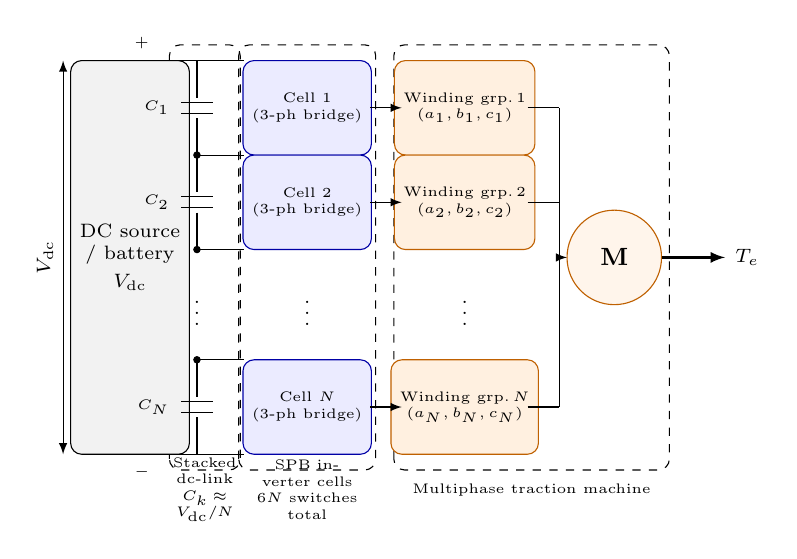
\begin{tikzpicture}[font=\scriptsize,>=latex,x=1mm,y=1mm]
% ---- styles ----
\tikzstyle{src}=[draw,rounded corners,align=center,fill=gray!10,
  minimum width=9mm,minimum height=50mm]
\tikzstyle{cellbox}=[draw=blue!65!black,rounded corners,align=center,
  fill=blue!8,minimum width=16mm,minimum height=12mm,font=\tiny]
\tikzstyle{windbox}=[draw=orange!75!black,rounded corners,align=center,
  fill=orange!12,minimum width=16mm,minimum height=12mm,font=\tiny]

% ---- group boxes (drawn first, underneath) ----
\draw[dashed,rounded corners] (9.5,-27) rectangle (18.5,27);
\draw[dashed,rounded corners] (18.3,-27) rectangle (35.7,27);
\draw[dashed,rounded corners] (38,-27) rectangle (73,27);

% ---- under-box labels ----
\node[font=\tiny,align=center,text width=9mm] at (14,-29.5)
  {Stacked dc-link\\$C_k\!\approx\!V_{\mathrm{dc}}/N$};
\node[font=\tiny,align=center,text width=17mm] at (27,-29.5)
  {SPB inverter cells\\$6N$ switches total};
\node[font=\tiny,align=center] at (55.5,-29.5)
  {Multiphase traction machine};

% ---- DC source ----
\node[src] (src) at (4.5,0) {DC source\\/ battery\\[2pt]$V_{\mathrm{dc}}$};
\draw[<->] (-4,-25) -- (-4,25);
\node[rotate=90] at (-6.3,0) {$V_{\mathrm{dc}}$};
\node[font=\tiny,anchor=south] at (6,25.3) {$+$};
\node[font=\tiny,anchor=north] at (6,-25.3) {$-$};

% ---- rails ----
\draw (9,25) -- (19,25);
\draw (9,-25) -- (19,-25);

% ---- stacked dc-link chain ----
\draw (13,25) -- (13,20.3);
\draw (11,19.7) -- (15,19.7);
\draw (11,18.3) -- (15,18.3);
\draw (13,17.7) -- (13,13);
\filldraw (13,13) circle (0.4);
\draw (13,13) -- (19,13);
\node[font=\tiny,anchor=east] at (10.7,19) {$C_1$};

\draw (13,13) -- (13,8.3);
\draw (11,7.7) -- (15,7.7);
\draw (11,6.3) -- (15,6.3);
\draw (13,5.7) -- (13,1);
\filldraw (13,1) circle (0.4);
\draw (13,1) -- (19,1);
\node[font=\tiny,anchor=east] at (10.7,7) {$C_2$};

\node[font=\scriptsize] at (13,-6) {$\vdots$};

\filldraw (13,-13) circle (0.4);
\draw (13,-13) -- (19,-13);
\draw (13,-13) -- (13,-17.7);
\draw (11,-18.3) -- (15,-18.3);
\draw (11,-19.7) -- (15,-19.7);
\draw (13,-20.3) -- (13,-25);
\node[font=\tiny,anchor=east] at (10.7,-19) {$C_N$};

% ---- SPB bridge cells ----
\node[cellbox] (c1) at (27,19) {Cell 1\\(3-ph bridge)};
\node[cellbox] (c2) at (27,7) {Cell 2\\(3-ph bridge)};
\node[font=\scriptsize] at (27,-6) {$\vdots$};
\node[cellbox] (cN) at (27,-19) {Cell $N$\\(3-ph bridge)};

% ---- winding groups ----
\node[windbox] (w1) at (47,19) {Winding grp.\,1\\$(a_1,b_1,c_1)$};
\node[windbox] (w2) at (47,7) {Winding grp.\,2\\$(a_2,b_2,c_2)$};
\node[font=\scriptsize] at (47,-6) {$\vdots$};
\node[windbox] (wN) at (47,-19) {Winding grp.\,$N$\\$(a_N,b_N,c_N)$};

\draw[->] (35,19) -- (39,19);
\draw[->] (35,7) -- (39,7);
\draw[->] (35,-19) -- (39,-19);

% ---- bus to machine ----
\draw (55,19) -- (59,19);
\draw (55,7) -- (59,7);
\draw (55,-19) -- (59,-19);
\draw (59,19) -- (59,-19);
\draw[->] (59,0) -- (60,0);

% ---- machine ----
\node[circle,draw=orange!75!black,fill=orange!8,minimum size=12mm,
  font=\bfseries\small] (M) at (66,0) {M};
\draw[->,thick] (M.east) -- ++(8,0) node[right,font=\scriptsize] {$T_e$};

\end{tikzpicture}}
    \caption{Conceptual architecture of an $N$-cell SPB traction
    drive. The dc source $V_{\mathrm{dc}}$ feeds $N$ series-connected
    local dc-link capacitors, each nominally $V_{\mathrm{dc}}/N$, that
    individually supply $N$ series-connected three-phase two-level
    bridge cells ($6N$ switches total); each cell drives one
    electrically separated three-phase winding group of the same
    machine, and the combined winding groups produce the
    electromagnetic torque $T_e$.}
    \label{fig:spb_architecture}
\end{figure}

SPB was introduced by Norrga \textit{et al.} for compact EV and HEV
drives \cite{Norrga2013SPB}; its subsequent development toward
higher-fidelity control, balancing, and reconfiguration is traced in
detail in Section~\ref{sec:evolution}.

Realizing this potential, however, introduces its own design
challenges: component count, dc-link dynamics, machine design,
common-mode voltage and insulation coordination, and fault handling
all become more tightly coupled, as examined in the sections that
follow, with thermal management identified as an open research
direction (Section~\ref{sec:future_directions}).

These questions have grown more relevant as neighboring research
areas have matured: multiphase machines provide additional
post-fault degrees of freedom, integrated modular motor drives show
how repeated power-electronic units can be physically associated with
individual machine sections, wide-bandgap semiconductors amplify
performance differences among voltage classes, and distributed
control coordinates modular converter units
\cite{Choi2011IMMD,Wang2025GaNIMMD,
JahnsDai2017IMDReview,Bringezu2020SPB,Deng2026IMDReview,
Ebrahimian2025GaNIMMD} -- together motivating SPB's assessment as a
complete converter--machine architecture rather than only a
series-connected topology.

Despite more than a decade of research on SPB, however, no study has
yet brought these threads together to systematically assess its
feasibility for electric-vehicle traction applications. The available
literature remains distributed across converter topology, modulation,
dc-link stability, multiphase-machine design, integrated motor drives,
semiconductor technology, thermal management, distributed control, and
fault-tolerant operation. Although these topics are strongly coupled
in an SPB traction drive, they are rarely evaluated within a common
system boundary. Moreover, most reported SPB experimental
demonstrations remain validated only at laboratory scale
(Section~\ref{sec:evolution}), even as the enabling
semiconductor, machine, cooling, and packaging technologies continue
to advance rapidly. This gap between a well-motivated architectural
concept and a system-level feasibility assessment is the gap that the
present paper addresses.

Accordingly, this paper provides a system-level review of SPB
traction-drive technology aimed at closing that gap. The remainder of
the paper is organized as follows. First, the historical development,
operating principle, and modulation of SPB are consolidated. Second,
the interaction between SPB cell count and the electric machine is
examined together with relevant multiphase-machine and integrated
modular motor-drive research, including the physical-integration and
insulation-coordination overhead introduced by series-connected
converter cells. Third, the series-stack origin of common-mode voltage
in SPB, its physical consequences, and mitigation options are
examined, followed by dc-link dynamics and balancing. Fourth,
semiconductor voltage scaling, SiC and GaN device selection, loss
scaling, and fault handling and reconfiguration are considered as
coupled architecture-level design problems. Finally, the research gaps
and requirements for high-power automotive validation are identified,
including high-power EMC validation and the quantitative comparison
against conventional two-level, multilevel, and cascaded alternatives
that remain open for future work.
% ============================================================================
\section{Evolution of the Stacked Polyphase Bridge Concept}
\label{sec:evolution}
% ============================================================================

This section traces how SPB's converter--machine modularity, together
with its associated control and modulation methods, has developed over
more than a decade of research, from an initial concept to an
increasingly reconfigurable and actively controlled
converter--machine system.

SPB emerged from a broader development toward modular converter--machine
systems. Earlier modular and integrated modular motor drives (IMMDs)
established the building blocks SPB later drew on, repeated
converter-winding modules, machine segmentation, power sharing, and
fault-tolerant operation \cite{Cengelci2000MMMI,Choi2011IMMD}, and
series-connected IMMD modules further showed that the total dc voltage
could be shared among inverter segments to enable lower-voltage
devices \cite{Wang2013GaNIMMD,Wang2025GaNIMMD}. A 2015 IEEE TIA study
by Wang, Li, and Han is especially relevant to SPB's later work,
combining series-connected GaN IMMD hardware with active cell-voltage
balancing and interleaved switching \cite{Wang2015GaNIMMD}.

Independent of this line of work, other series-connected modular
motor-drive topologies were proposed with the same underlying
dc-voltage-sharing principle \cite{Wang2015SeriesModular,
Ruseler2015InputSeries}, indicating that the concept was not unique
to SPB but part of a broader convergence toward series-connected
modularity. A related KTH comparative study evaluated SPB alongside
other integrated modular converter candidates for traction
drives, the parallel-connected polyphase bridge converter (PPB-I, a
conventional multiphase converter with phase-leg-level modularity, and
PPB-II, several interleaved two-level three-phase converters each with
its own dc capacitor) and the modular high-frequency (MHF) converter,
against a conventional two-level three-phase drive as a baseline in
terms of machine design, losses, capacitor energy storage, cost, and
redundancy, confirming that SPB is one of several modular-converter
topology candidates studied for this application
\cite{Zhang2017ModularDriveComparison}.

Building on this foundation, the SPB topology itself was introduced in
2013 \cite{Norrga2013SPB}, followed shortly thereafter by dedicated
control and modulation work \cite{Jin2014Control}. Related series-connected multiphase drives
demonstrated that machine-side degrees of freedom could be used to
regulate internal dc-link voltage sharing \cite{Che2014SeriesConnected},
while Nikouie \textit{et al.} formally established the SPB dc-link
stability problem and the corresponding balancing-controller
requirements \cite{Nikouie2015Stability,Nikouie2017Stability}. This
period established the topology's basic feasibility and identified
dc-link voltage balancing, rather than semiconductor voltage rating
alone, as its first-order control challenge.

The next stage of development shifted the focus toward modulation,
scalable control, and converter--machine co-design: modulation was
shown to directly influence semiconductor loss and dc-link harmonic
content \cite{Jin2017Modulation}, distributed control offered an
alternative to centralized balancing \cite{Jin2018Distributed}, and
interleaving and phase-count studies tied converter design to machine
architecture \cite{Verkroost2019Interleaving,VanDamme2019DCLink,
Bringezu2020SPB,Verkroost2021Ripple}. Collectively, this reframed SPB
from a series-connected converter topology into a converter--machine
co-design problem in which modulation, control, and machine parameters
jointly determine dc-link behavior.

More recent work has moved from repeated but statically configured
hardware toward actively reconfigurable modular systems.
Common-duty-ratio operation, decentralized voltage balancing, and
multi-agent power distribution have reduced the dependence on
centralized control \cite{Mocevic2023CDR,Verkroost2024VoltageBalance,
Verkroost2024PowerDistribution,Mocevic2024GateDelay}. Online module
isolation and reintroduction have further demonstrated dynamic dc-bus
reconfiguration, removing a faulted cell without interrupting torque
production \cite{Verkroost2024Reconfiguration}.
In parallel, modern GaN devices have renewed interest in SPB as a
route to lower semiconductor voltage classes in integrated drives
\cite{Rohner2024GaN}.

Fig.~\ref{fig:spb_timeline} places representative milestones from
across these stages on a chronological timeline of the topology's
development, together with the validation level, reported scale, and
the specific implication each result carries for the system-level
review developed in this paper.

\begin{figure}[!t]
\centering
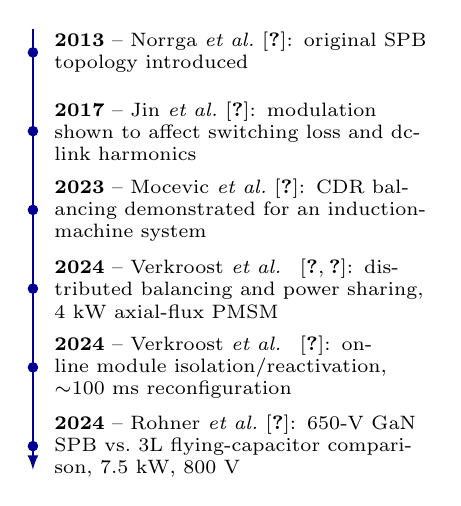
\begin{tikzpicture}[font=\scriptsize,>=latex]
\tikzstyle{yr}=[circle,draw=blue!65!black,fill=blue!55!black,inner sep=1.2pt]
\tikzstyle{txt}=[align=left,text width=48mm,inner sep=0pt]
\draw[->,thick,blue!55!black] (0,3mm) -- (0,-53mm);
\node[yr] (n1) at (0,0mm) {};
\node[txt,right=2mm of n1]
{\textbf{2013} -- Norrga \textit{et al.}~\cite{Norrga2013SPB}:
original SPB topology introduced};
\node[yr] (n2) at (0,-10mm) {};
\node[txt,right=2mm of n2]
{\textbf{2017} -- Jin \textit{et al.}~\cite{Jin2017Modulation}:
modulation shown to affect switching loss and dc-link harmonics};
\node[yr] (n3) at (0,-20mm) {};
\node[txt,right=2mm of n3]
{\textbf{2023} -- Mocevic \textit{et al.}~\cite{Mocevic2023CDR}:
CDR balancing demonstrated for an induction-machine system};
\node[yr] (n4) at (0,-30mm) {};
\node[txt,right=2mm of n4]
{\textbf{2024} -- Verkroost \textit{et al.}
~\cite{Verkroost2024VoltageBalance,Verkroost2024PowerDistribution}:
distributed balancing and power sharing, 4~kW axial-flux PMSM};
\node[yr] (n5) at (0,-40mm) {};
\node[txt,right=2mm of n5]
{\textbf{2024} -- Verkroost \textit{et al.}
~\cite{Verkroost2024Reconfiguration}: online module
isolation/reactivation, $\sim$100~ms reconfiguration};
\node[yr] (n6) at (0,-50mm) {};
\node[txt,right=2mm of n6]
{\textbf{2024} -- Rohner \textit{et al.}~\cite{Rohner2024GaN}:
650-V GaN SPB vs.\ 3L flying-capacitor comparison, 7.5~kW, 800~V};
\end{tikzpicture}
\caption{Chronological milestones in SPB research, from the original
topology through modulation, distributed balancing, reconfiguration,
and wide-bandgap integration.}
\label{fig:spb_timeline}
\end{figure}

As Fig.~\ref{fig:spb_timeline} indicates, this progression has been
validated primarily at laboratory scale, typically at or below several
kilowatts, leaving open whether the demonstrated control, balancing,
and reconfiguration principles extend to the automotive and heavy-duty
power levels summarized in Table~\ref{tab:intro_voltage_power} -- a
gap revisited throughout the remainder of this paper.
% ============================================================================
\section{Operating Principle and Topological Characteristics}
\label{sec:operating_principle}
% ============================================================================

This section formalizes the operating principle underlying SPB's two
coupled properties -- reduced semiconductor voltage stress and
converter--machine modularity -- and establishes the notation and
voltage/power relations used throughout the remainder of the paper.

\subsection{Basic Structure and Voltage Partitioning}

An $N$-cell SPB consists of $N$ conventional three-phase two-level
voltage-source inverter cells connected in series on the dc side, with
each bridge supplying one electrically separated three-phase winding
group of the same machine \cite{Norrga2013SPB,Jin2014Control,
Jin2017Modulation}. The machine therefore presents $N$ ac ports, while
the converter cells share a single series dc path. This structure is
the physical implementation of the voltage-partitioning principle
introduced in Section~\ref{sec:semiconductor_limitations}.

The dc-link voltage satisfies

\begin{equation}
V_{\mathrm{dc}}=\sum_{k=1}^{N}V_{\mathrm{dc},k},
\qquad
V_{\mathrm{dc},k}\approx\frac{V_{\mathrm{dc}}}{N}
\label{eq:spb_voltage_sum}
\end{equation}

under balanced operation. A basic implementation contains $6N$ active
switches and $N$ local dc-link capacitors. Increasing $N$ therefore
reduces the nominal cell voltage, and hence the required semiconductor
voltage class, but simultaneously increases the number of switches,
gate drivers, sensors, capacitors, and machine-winding terminals that
must be realized and managed. This tradeoff between semiconductor
voltage rating and component count is quantified further in
Section~\ref{sec:semiconductor_scaling} and is revisited from a
machine-design perspective below. Fig.~\ref{fig:spb_switch_schematic}
shows this structure at switch level for two representative cells,
making explicit the $6N$-switch bridge realization, the local
capacitors $C_k$, and the notation used throughout the remainder of
this paper.

\begin{figure}[!t]
\centering
\resizebox{\columnwidth}{!}{%
\begin{circuitikz}[font=\scriptsize, x=1mm, y=1mm, >=latex]
\ctikzset{bipoles/length=5mm}

% ---- dc source (3-cell battery-pack symbol) ----
\draw (-10,10.5) -- (-10,28) -- (-4.5,28) -- (0,28);
\draw (-10,-10.5) -- (-10,-28) -- (-4.5,-28) -- (0,-28);
\draw (-10,10.5) to[battery1] (-10,3.5) to[battery1] (-10,-3.5)
  to[battery1] (-10,-10.5);
\node[font=\tiny] at (-5.3,0) {$V_{\mathrm{dc}}$};
\draw[<->] (-19,-28) -- (-19,28);
\node[rotate=90] at (-21.3,0) {$V_{\mathrm{dc}}$};
\node[font=\tiny,anchor=south] at (-4.5,28.3) {$+$};
\node[font=\tiny,anchor=north] at (-4.5,-28.3) {$-$};

% ---- series dc backbone (elided cells 2..N-1) ----
\draw (0,16) -- (0,9);
\node[font=\scriptsize] at (0,0) {$\vdots$};
\draw (0,-9) -- (0,-16);

% ---- series dc current ----
\draw[->,thick] (-2.3,25) -- (-2.3,19);
\node[font=\tiny,anchor=east] at (-2.7,22) {$i_{\mathrm{dc}}$};

% ================= CELL 1 =================
\node[font=\tiny] at (21,31.8) {Cell 1};
\draw (0,28) -- (40,28);
\draw (0,16) -- (40,16);
\draw (6,28) to[C, l=$C_1$] (6,16);
\node[font=\tiny,align=center] at (21,12.5) {$V_{\mathrm{dc},1}\approx V_{\mathrm{dc}}/N$};

\draw (13,28) to[nos] (13,22);
\draw (13,22) to[nos] (13,16);
\draw (21,28) to[nos] (21,22);
\draw (21,22) to[nos] (21,16);
\draw (29,28) to[nos] (29,22);
\draw (29,22) to[nos] (29,16);

\draw (13,22) -- (15.5,22) node[right=1pt,font=\tiny] {$a_1$};
\draw (21,22) -- (23.5,22) node[right=1pt,font=\tiny] {$b_1$};
\draw (29,22) -- (31.5,22) node[right=1pt,font=\tiny] {$c_1$};

% ---- star (wye) winding group 1, local neutral n_1 ----
% three separate lanes (well-separated in y) carry each phase's
% winding coil, converging only in a short diagonal stub at the end
% so the three coils remain visually distinct rather than bunching.
\draw[orange!70!black] (15.5,22) -- (15.5,26) -- (40,26);
\draw[orange!70!black] (40,26) to[cute inductor] (46,26);
\draw[orange!70!black] (46,26) -- (52,22);
\draw[orange!70!black] (23.5,22) -- (23.5,18) -- (40,18);
\draw[orange!70!black] (40,18) to[cute inductor] (46,18);
\draw[orange!70!black] (46,18) -- (52,22);
\draw[orange!70!black] (31.5,22) -- (40,22);
\draw[orange!70!black] (40,22) to[cute inductor] (46,22);
\draw[orange!70!black] (46,22) -- (52,22);
\node[circle,fill=orange!70!black,inner sep=0.5pt] at (52,22) {};
\node[font=\tiny,anchor=west,orange!70!black] at (53.3,22) {$n_1$};

\draw[->,blue!55!black] (2,31) -- (2,28.3);
\node[font=\tiny,anchor=south,blue!55!black] at (2,31.2) {$p_{\mathrm{dc},1}$};

% ================= elided cells =================
\node[font=\tiny,align=center] at (21,0) {(cells $2,\dots,N\!-\!1$\\elided)};
\node[font=\scriptsize] at (50,0) {$\vdots$};

% ================= CELL N =================
\node[font=\tiny] at (21,-31.8) {Cell $N$};
\draw (0,-16) -- (40,-16);
\draw (0,-28) -- (40,-28);
\draw (6,-16) to[C, l=$C_N$] (6,-28);
\node[font=\tiny,align=center] at (21,-12.5) {$V_{\mathrm{dc},N}\approx V_{\mathrm{dc}}/N$};

\draw (13,-16) to[nos] (13,-22);
\draw (13,-22) to[nos] (13,-28);
\draw (21,-16) to[nos] (21,-22);
\draw (21,-22) to[nos] (21,-28);
\draw (29,-16) to[nos] (29,-22);
\draw (29,-22) to[nos] (29,-28);

\draw (13,-22) -- (15.5,-22) node[right=1pt,font=\tiny] {$a_N$};
\draw (21,-22) -- (23.5,-22) node[right=1pt,font=\tiny] {$b_N$};
\draw (29,-22) -- (31.5,-22) node[right=1pt,font=\tiny] {$c_N$};

% ---- star (wye) winding group N, local neutral n_N ----
% mirrored version of the Cell 1 lane layout above.
\draw[orange!70!black] (15.5,-22) -- (15.5,-26) -- (40,-26);
\draw[orange!70!black] (40,-26) to[cute inductor] (46,-26);
\draw[orange!70!black] (46,-26) -- (52,-22);
\draw[orange!70!black] (23.5,-22) -- (23.5,-18) -- (40,-18);
\draw[orange!70!black] (40,-18) to[cute inductor] (46,-18);
\draw[orange!70!black] (46,-18) -- (52,-22);
\draw[orange!70!black] (31.5,-22) -- (40,-22);
\draw[orange!70!black] (40,-22) to[cute inductor] (46,-22);
\draw[orange!70!black] (46,-22) -- (52,-22);
\node[circle,fill=orange!70!black,inner sep=0.5pt] at (52,-22) {};
\node[font=\tiny,anchor=west,orange!70!black] at (53.3,-22) {$n_N$};

\draw[->,blue!55!black] (2,-13) -- (2,-16.3);
\node[font=\tiny,anchor=south,blue!55!black] at (2,-12.8) {$p_{\mathrm{dc},N}$};

\end{circuitikz}}
\caption{Switch-level realization of the SPB dc--ac stage for two
representative cells (Cell~1 and Cell~$N$; cells $2,\dots,N-1$
elided). Each cell is a conventional two-level three-phase bridge
(six switches per cell, $6N$ total) fed from its own local dc-link
capacitor $C_k$, with leg midpoints $a_k,b_k,c_k$ feeding a
star-connected winding group $k$ at its own electrically separate
neutral point $n_k$ (only $n_1$ and $n_N$ shown; the star points are
not interconnected). The common series current $i_{\mathrm{dc}}$
\eqref{eq:series_current} flows through every cell, giving each cell
the dc-side power $p_{\mathrm{dc},k}=V_{\mathrm{dc},k}i_{\mathrm{dc}}$
\eqref{eq:cell_dc_power}.}
\label{fig:spb_switch_schematic}
\end{figure}

\subsection{Series DC Connection and Power Flow}

The defining structural difference between SPB and parallel modular
drives is the series dc connection. Neglecting auxiliary and bypass
paths, the cell dc currents are constrained to be equal,

\begin{equation}
i_{\mathrm{dc},1}=i_{\mathrm{dc},2}=\cdots=i_{\mathrm{dc},N}
=i_{\mathrm{dc}},
\label{eq:series_current}
\end{equation}

so that the dc-side power entering cell $k$ is

\begin{equation}
p_{\mathrm{dc},k}=V_{\mathrm{dc},k}i_{\mathrm{dc}}.
\label{eq:cell_dc_power}
\end{equation}

The total machine power, by contrast, is the sum of the powers
delivered to the individual winding groups,

\begin{equation}
P_{\mathrm{ac}}=\sum_{k=1}^{N}P_k.
\label{eq:power_sum}
\end{equation}

Under symmetrical operation $P_k\approx P_{\mathrm{ac}}/N$, but equal
power sharing is not a fundamental requirement of the topology. The
multi-three-phase machine provides additional current and power
degrees of freedom that allow power to be redistributed among winding
groups while the required total torque is maintained
\cite{Che2014SeriesConnected,Verkroost2024PowerDistribution}. This
redistribution capability is the physical basis for both dc-link
voltage balancing and several of the post-fault operating strategies
discussed in later sections.

The combination of a common dc current with independently
controllable ac-side powers also explains why the local capacitor
voltages must be treated as internal dynamic states rather than fixed
design parameters. If one winding group processes more power than
another, the corresponding capacitor energies can diverge even though
all cells carry the same dc current \cite{Nikouie2015Stability,
Nikouie2017Stability}. Managing this divergence is precisely the
dc-link stability and balancing problem identified in
Section~\ref{sec:evolution} as the topology's first-order control
challenge.

\subsection{SPB as an Input-Series, Multi-Three-Phase-Output Drive}

These relations place SPB in a distinct category relative to the
conventional multilevel converters discussed in
Section~\ref{sec:introduction}, which partition dc-link voltage
internally while retaining a conventional three-phase machine. In
SPB, by contrast, each converter cell remains a standard two-level
bridge, and it is the machine itself that provides the multiple ac
ports required to transfer power out of the series dc stack. SPB can
therefore be characterized as an \emph{input-series,
multi-three-phase-output} drive, a description that makes explicit
why voltage partitioning in SPB cannot be separated from machine
design.

\subsection{Cell Count as a Converter--Machine Design Variable}

Cell count is consequently a converter--machine design variable rather
than a semiconductor variable alone. As established above, increasing
$N$ also reduces the voltage available to each winding group and
alters the number of winding sets, terminal count, electromagnetic
coupling, current-control degrees of freedom, and available
reconfiguration states. Bringezu and
Biela demonstrated this interaction directly by comparing SPB systems
based on 3-, 6-, 9-, and 12-phase PMSMs \cite{Bringezu2020SPB}.

A related and often overlooked point is that machine phase current
does not generally scale as $1/N$. The required phase current instead
depends on the number of turns, flux linkage, winding connection,
torque constant, and machine geometry. A many-cell architecture may
therefore reduce the semiconductor voltage class while still requiring
high-current devices or parallel chips at the device level. This
coupling between cell count, voltage class, and current rating is
particularly important when the comparison is extended from
high-voltage SiC implementations toward lower-voltage GaN
implementations, as considered in Section~\ref{sec:semiconductor_limitations}.

% ============================================================================
\section{Electric-Machine Requirements and Integrated Implementation}
\label{sec:machine_requirements}
% ============================================================================

% ---------------------------------------------------------------------------
\subsection{Winding Architecture and Electromagnetic Coupling}
% ---------------------------------------------------------------------------

Although the winding groups are electrically separated at their
terminals, they share the same magnetic circuit, rotor, air gap, and
shaft. 
Their electromagnetic coupling depends on winding distribution,
slot/pole combination, spatial displacement, and machine geometry
\cite{Che2014SeriesConnected,Bringezu2020SPB,
Verkroost2024PowerDistribution,Zhang2014SPBMachine}. 
Therefore, an SPB-compatible machine
cannot generally be obtained simply by dividing a conventional
three-phase winding into multiple groups without considering the
resulting coupling and harmonic behavior.

The three-phase groups may be aligned, 
spatially shifted, or implemented as physically segmented stator
modules. 
Spatial displacement affects mutual coupling, torque-ripple
components, and the additional current subspaces available to the
controller, among other effects
\cite{Zhang2025MultiphaseReview,Das2025SixPhaseWinding,
Wang2025DTPHarmonics}. 
These additional subspaces can introduce non-torque-producing currents,
 but they can also be exploited for
harmonic suppression, differential power sharing, and fault-tolerant
operation
\cite{Tang2025SixPhaseFault,Verkroost2024PowerDistribution}. 
Split winding architectures show a similar tradeoff: they can reduce ripple
and provide additional current/voltage degrees of freedom, but they do
so by increasing winding terminals and coupling complexity
\cite{Han2014SplitWindingModular}. These three winding-group
arrangements are compared schematically in
Fig.~\ref{fig:winding_options}.

\begin{figure*}[!t]
\centering
\resizebox{\textwidth}{!}{%
\begin{circuitikz}[font=\scriptsize,>=latex,x=1mm,y=1mm]
\ctikzset{bipoles/length=4mm}

% =====================================================================
% Panel (a): Aligned -- every slot hosts both groups, inner/outer layer.
% Long coil legs reaching close to the bore boundary and a shaft-only
% center marker (not a large rotor disk) so the content, not empty
% space, dominates the circle -- matching the reference proportions.
% =====================================================================
\begin{scope}[shift={(0,0)}]
\draw[fill=black!25] (0,0) circle (2.2);
\draw[black!40,thin] (0,0) circle (52);
\foreach \a in {90,210,330}{
\draw[black!20,thin] (\a:3) -- (\a:50.5);
\begin{scope}[shift={(\a:22)}]
\foreach \la/\lb in {90/A,210/B,330/C}{
  \draw[blue!55!black,ultra thick] (\la:1.2) to[cute inductor] (\la:9);
  \node[font=\small,blue!55!black] at (\la:11) {$\lb$1};
}
\node[circle,fill=blue!55!black,inner sep=0.8pt] at (0,0) {};
\end{scope}
\begin{scope}[shift={(\a:38)}]
\foreach \la/\lb in {90/A,210/B,330/C}{
  \draw[orange!70!black,ultra thick] (\la:1.2) to[cute inductor] (\la:9);
  \node[font=\small,orange!70!black] at (\la:11) {$\lb$2};
}
\node[circle,fill=orange!70!black,inner sep=0.8pt] at (0,0) {};
\end{scope}
}
\node[align=center] at (0,-60) {(a) Aligned};
\end{scope}

% =====================================================================
% Panel (b): Shifted -- both groups at the same radius, offset by
% Delta-theta so the six coil clusters interleave with long legs
% reaching close to the boundary
% =====================================================================
\begin{scope}[shift={(102,0)}]
\draw[fill=black!25] (0,0) circle (2.2);
\draw[black!40,thin] (0,0) circle (39);
\foreach \a in {90,210,330}{
\begin{scope}[shift={(\a:26)}]
\foreach \la/\lb in {90/A,210/B,330/C}{
  \draw[blue!55!black,ultra thick] (\la:1.2) to[cute inductor] (\la:9);
  \node[font=\small,blue!55!black] at (\la:11) {$\lb$1};
}
\node[circle,fill=blue!55!black,inner sep=0.8pt] at (0,0) {};
\end{scope}
\pgfmathsetmacro{\ashift}{\a+60}
\begin{scope}[shift={(\ashift:26)}]
\foreach \la/\lb in {90/A,210/B,330/C}{
  \draw[orange!70!black,ultra thick] (\la:1.2) to[cute inductor] (\la:9);
  \node[font=\small,orange!70!black] at (\la:11) {$\lb$2};
}
\node[circle,fill=orange!70!black,inner sep=0.8pt] at (0,0) {};
\end{scope}
}
\draw[->,thin,black!60] (120:36) arc[start angle=120,end angle=150,radius=36];
\node[font=\small] at (135:39) {$\Delta\theta$};
\node[align=center] at (0,-47) {(b) Shifted};
\end{scope}

% =====================================================================
% Panel (c): Segmented -- one shared bore, split into four physically
% separate modules (dashed radial boundaries) alternating group 1 and
% group 2, with the same long-leg coil size as (a)/(b)
% =====================================================================
\begin{scope}[shift={(204,0)}]
\draw[fill=black!25] (0,0) circle (2.2);
\draw[black!40,thin] (0,0) circle (39);
\foreach \b in {45,135,225,315}{
  \draw[black!40,thin,dashed] (\b:3) -- (\b:37.5);
}
\begin{scope}[shift={(0:26)}]
\foreach \la/\lb in {90/A1,210/B1,330/C1}{
  \draw[blue!55!black,ultra thick] (\la:1.2) to[cute inductor] (\la:9);
  \node[font=\small,blue!55!black] at (\la:11) {$\lb$};
}
\node[circle,fill=blue!55!black,inner sep=0.8pt] at (0,0) {};
\end{scope}
\begin{scope}[shift={(180:26)}]
\foreach \la/\lb in {90/A1,210/B1,330/C1}{
  \draw[blue!55!black,ultra thick] (\la:1.2) to[cute inductor] (\la:9);
  \node[font=\small,blue!55!black] at (\la:11) {$\lb$};
}
\node[circle,fill=blue!55!black,inner sep=0.8pt] at (0,0) {};
\end{scope}
\begin{scope}[shift={(90:26)}]
\foreach \la/\lb in {90/A2,210/B2,330/C2}{
  \draw[orange!70!black,ultra thick] (\la:1.2) to[cute inductor] (\la:9);
  \node[font=\small,orange!70!black] at (\la:11) {$\lb$};
}
\node[circle,fill=orange!70!black,inner sep=0.8pt] at (0,0) {};
\end{scope}
\begin{scope}[shift={(270:26)}]
\foreach \la/\lb in {90/A2,210/B2,330/C2}{
  \draw[orange!70!black,ultra thick] (\la:1.2) to[cute inductor] (\la:9);
  \node[font=\small,orange!70!black] at (\la:11) {$\lb$};
}
\node[circle,fill=orange!70!black,inner sep=0.8pt] at (0,0) {};
\end{scope}
\node[align=center] at (0,-47) {(c) Segmented};
\end{scope}

% ---- Legend ----
\node[circle,fill=blue!55!black,inner sep=1.4pt] at (72,-70) {};
\node[right,font=\small] at (73.8,-70) {Winding group 1};
\node[circle,fill=orange!70!black,inner sep=1.4pt] at (127,-70) {};
\node[right,font=\small] at (128.8,-70) {Winding group 2};
\node[fill=black!25,minimum size=2mm,inner sep=0] at (10,-70) {};
\node[right,font=\small] at (11.8,-70) {Shaft};
\end{circuitikz}}
\caption{Schematic comparison of the winding-group spatial arrangements
: (a)~aligned  groups (b)~spatially shifted groups and (c)~physically
segmented stator modules.}
\label{fig:winding_options}
\end{figure*}

For the $k$th PMSM winding group,

\begin{equation}
\begin{aligned}
v_{d,k}&=R_{s,k}i_{d,k}-\omega_{\mathrm e}L_{q,k}i_{q,k},\\
v_{q,k}&=R_{s,k}i_{q,k}
+\omega_{\mathrm e}\left(L_{d,k}i_{d,k}+\psi_{f,k}\right),
\end{aligned}
\label{eq:spb_machine_dq}
\end{equation}

and the required voltage must satisfy

\begin{equation}
\sqrt{v_{d,k}^{2}+v_{q,k}^{2}}
\leq
k_{\mathrm{mod}}V_{\mathrm{dc},k}
\approx
k_{\mathrm{mod}}\frac{V_{\mathrm{dc}}}{N}.
\label{eq:spb_machine_voltage_limit}
\end{equation}

This falling per-cell voltage budget ties winding turns, inductance,
and field-weakening capability directly to $N$ -- a coupling
demonstrated in optimized multiphase SPB-PMSM systems
\cite{Bringezu2020SPB}. Recent multiphase traction-machine studies
similarly emphasize coordinated design of winding voltage, harmonic
subspaces, and modulation
\cite{Chen2026HighModulationDTP,Feng2026TractionMachine}.

% ---------------------------------------------------------------------------
\subsection{From Multiphase Machine to Integrated Modular Drive}
% ---------------------------------------------------------------------------

Physical integration can convert the added electrical complexity of
many winding groups into a packaging advantage. With a remote
inverter, additional winding groups increase phase-cable and connector
count; positioning each converter bridge close to its corresponding
winding group instead reduces external cabling, shortens
high-frequency interconnections, distributes heat sources, and aligns
converter modules with stator segments.

This design philosophy predates SPB and has been extensively studied
in integrated and modular motor drives
\cite{Shakweh2002PlugPlayIMD,Wheeler2005Integrated30kW,
Pickering2006ThermalIMD,Brown2007IMMD,Wolmarans2008IntegratedFT,
Hennen2012DistributedIMMD,Choi2011IMMD,Wang2013GaNIMMD,
Wang2015GaNIMMD,Wang2025GaNIMMD,Ugur2018GaNIMMD,
Ugur2019MultiphysicsIMMD,Mohamed2021Electrothermal,
Mohamed2021EnhancedIMD,Mohamed2022IntegratedDCLink,Wang2025MWIMMD,
Chen2026WBGIMD,Deng2026IMDReview}, summarized in
Table~\ref{tab:immd_relevance}. The overall trend runs from early
cable-reduction and compact-packaging concepts through jointly
designed fault-tolerant converter/winding/thermal architectures and
series-connected GaN IMMDs to recent WBG-based axial-flux IMMDs
demonstrating stator-mounted converter modules and scalability to
MW-class and EV-traction implementations.

% ---------------------------------------------------------------------------
\subsection{Physical Integration Options}
\label{subsec:physical_integration}
% ---------------------------------------------------------------------------

The electrically separated winding groups required by SPB do not
impose a unique converter placement on a radial-flux machine. Chowdhury
\textit{et al.} \cite{Chowdhury2019Integration}, consistent with the
broader integrated-motor-drive survey of Abebe \textit{et al.}
\cite{Abebe2016IMDReview}, classify motor/inverter physical integration
into four categories: whether the converter mounts radially or
axially, and whether it interfaces with a separate housing/end-cap
structure or directly with the stator core. This taxonomy frames how
SPB converter cells can be placed around a radial-flux machine, as
illustrated in Fig.~\ref{fig:machine_integration}. The axial-flux
stator-mounted and polygon-housing alternative is covered by the
Mohamed \textit{et al.} developments
\cite{Mohamed2021Electrothermal,Mohamed2021EnhancedIMD,
Mohamed2022IntegratedDCLink} in Table~\ref{tab:immd_relevance}.


%\cite{Abebe2015FEAThermal}.

\begin{figure*}[!t]
\centering
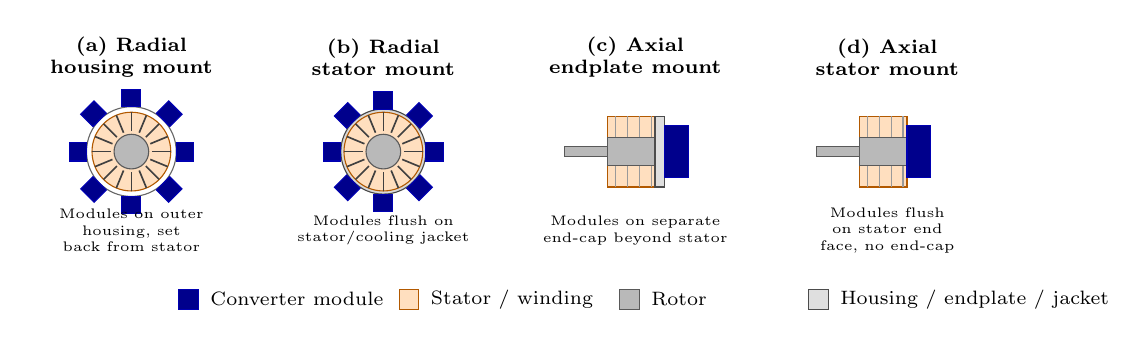
\begin{tikzpicture}[font=\scriptsize,>=latex,x=1mm,y=1mm]
% ================= Panel (a): Radial housing mount (radial cross-section) =================
\begin{scope}[shift={(0,0)}]
\draw[fill=orange!25,draw=orange!70!black,thin] (0,0) circle (5);
\foreach \a in {0,22.5,...,337.5}{\draw[black!75,semithick] (\a:2.6) -- (\a:5);}
\draw[fill=gray!55,draw=gray!70!black,thin] (0,0) circle (2.2);
\draw[black!60,thin] (0,0) circle (5.7);
\foreach \a in {0,45,90,135,180,225,270,315}{
  \begin{scope}[rotate=\a]
    \draw[fill=blue!55!black,draw=blue!70!black,thin] (5.7,-1.2) rectangle (7.9,1.2);
  \end{scope}
}
\end{scope}
\node[font=\scriptsize\bfseries,align=center] at (0,12) {(a) Radial\\housing mount};
\node[font=\tiny,align=center,text width=24mm] at (0,-10)
  {Modules on outer housing, set back from stator};

% ================= Panel (b): Radial stator mount (radial cross-section) =================
\begin{scope}[shift={(32,0)}]
\draw[fill=gray!30,draw=gray!55!black,thin] (0,0) circle (5.4);
\draw[fill=orange!25,draw=orange!70!black,thin] (0,0) circle (5);
\foreach \a in {0,22.5,...,337.5}{\draw[black!75,semithick] (\a:2.6) -- (\a:5);}
\draw[fill=gray!55,draw=gray!70!black,thin] (0,0) circle (2.2);
\foreach \a in {0,45,90,135,180,225,270,315}{
  \begin{scope}[rotate=\a]
    \draw[fill=blue!55!black,draw=blue!70!black,thin] (5.4,-1.2) rectangle (7.6,1.2);
  \end{scope}
}
\end{scope}
\node[font=\scriptsize\bfseries,align=center] at (32,12) {(b) Radial\\stator mount};
\node[font=\tiny,align=center,text width=24mm] at (32,-10)
  {Modules flush on stator/cooling jacket};

% ================= Panel (c): Axial endplate mount (axial cross-section) =================
\begin{scope}[shift={(64,0)}]
\draw[fill=orange!25,draw=orange!70!black,thin] (-3.5,-4.5) rectangle (2.5,4.5);
\foreach \x in {-2.5,-1,0.5,2}{\draw[black!40,thin] (\x,-4.5) -- (\x,4.5);}
\draw[fill=gray!55,draw=gray!70!black,thin] (-3.5,-1.8) rectangle (2.5,1.8);
\draw[fill=gray!55,draw=gray!70!black,thin] (-9,-0.6) rectangle (-3.5,0.6);
\draw[fill=gray!25,draw=gray!60!black,thin] (2.5,-4.5) rectangle (3.7,4.5);
\draw[fill=blue!55!black,draw=blue!70!black,thin] (3.7,-3.3) rectangle (6.7,3.3);
\end{scope}
\node[font=\scriptsize\bfseries,align=center] at (64,12) {(c) Axial\\endplate mount};
\node[font=\tiny,align=center,text width=24mm] at (64,-10)
  {Modules on separate end-cap beyond stator};

% ================= Panel (d): Axial stator mount (axial cross-section) =================
\begin{scope}[shift={(96,0)}]
\draw[fill=orange!25,draw=orange!70!black,thin] (-3.5,-4.5) rectangle (2.5,4.5);
\foreach \x in {-2.5,-1,0.5,2}{\draw[black!40,thin] (\x,-4.5) -- (\x,4.5);}
\draw[fill=gray!55,draw=gray!70!black,thin] (-3.5,-1.8) rectangle (2.5,1.8);
\draw[fill=gray!55,draw=gray!70!black,thin] (-9,-0.6) rectangle (-3.5,0.6);
\draw[fill=blue!55!black,draw=blue!70!black,thin] (2.5,-3.3) rectangle (5.5,3.3);
\end{scope}
\node[font=\scriptsize\bfseries,align=center] at (96,12) {(d) Axial\\stator mount};
\node[font=\tiny,align=center,text width=24mm] at (96,-10)
  {Modules flush on stator end face, no end-cap};

% ================= Legend =================
\draw[fill=blue!55!black,draw=blue!70!black,thin] (6,-20) rectangle (8.5,-17.5);
\node[right] at (8.8,-18.75) {Converter module};
\draw[fill=orange!25,draw=orange!70!black,thin] (34,-20) rectangle (36.5,-17.5);
\node[right] at (36.8,-18.75) {Stator / winding};
\draw[fill=gray!55,draw=gray!70!black,thin] (62,-20) rectangle (64.5,-17.5);
\node[right] at (64.8,-18.75) {Rotor};
\draw[fill=gray!25,draw=gray!60!black,thin] (86,-20) rectangle (88.5,-17.5);
\node[right] at (88.8,-18.75) {Housing / endplate / jacket};
\end{tikzpicture}
\caption{Physical integration options for SPB-compatible converter
modules on a radial-flux machine, following the four-category
taxonomy of \cite{Chowdhury2019Integration}: (a) radial housing mount,
(b) radial stator mount, (c) axial endplate mount, and (d) axial
stator mount, each shown in whichever radial or axial cross-section
most clearly conveys its mounting geometry.}
\label{fig:machine_integration}
\end{figure*}

\begin{table}[!t]
\centering
\caption{Representative Integrated Motor-Drive
Developments}
\label{tab:immd_relevance}
\footnotesize
\renewcommand{\arraystretch}{1.05}
\setlength{\tabcolsep}{4pt}
\begin{tabular}{p{2.3cm}p{5.3cm}}
\hline
\textbf{Reference} & \textbf{Integration theme}\\
\hline

Shakweh \textit{et al.} \cite{Shakweh2002PlugPlayIMD} &
Integrated motor/inverter architecture\\

Wheeler/Pickering \textit{et al.}
\cite{Wheeler2005Integrated30kW,Pickering2006ThermalIMD} &
Converter and thermal design inside motor envelope\\

Brown \textit{et al.} \cite{Brown2007IMMD} &
Converter mounted at modular stator pole\\

Wolmarans \textit{et al.} \cite{Wolmarans2008IntegratedFT} &
Fault-tolerant converter, machine, and thermal design\\

Choi \textit{et al.} \cite{Choi2011IMMD} &
Modular PM machine and high-temperature electronics\\

Wang \textit{et al.}
\cite{Wang2013GaNIMMD,Wang2025GaNIMMD} &
Low-voltage GaN, dc-voltage sharing, and interleaving\\

U\u{g}ur and Keysan
\cite{Ugur2018GaNIMMD,Ugur2019MultiphysicsIMMD} &
Multi-physics converter--machine optimization\\

Mohamed \textit{et al.}
\cite{Mohamed2021Electrothermal,
Mohamed2021EnhancedIMD,Mohamed2022IntegratedDCLink} &
Stator-mounted modules, polygon housing, integrated dc link\\

Wang \textit{et al.} \cite{Wang2025MWIMMD} &
Repeated machine and converter submodules\\

Chen \textit{et al.} \cite{Chen2026WBGIMD} &
WBG converter, machine, passive, and cooling co-design\\

Deng \textit{et al.} \cite{Deng2026IMDReview} &
Recent IMD technologies and research directions\\
\hline
\end{tabular}
\end{table}

Modern WBG drives therefore provide several machine and packaging
concepts that are compatible with SPB, including segmented windings,
distributed converter cells, shared cooling, and integrated dc-link
structures. These developments do not establish an intrinsic SPB
advantage, but they demonstrate the availability of enabling
technologies required for practical implementation.

% ---------------------------------------------------------------------------
\subsection{Integration Is Not Free of Complexity}
% ---------------------------------------------------------------------------

Integration does not remove complexity; it relocates it. Converter
modules mounted on or near the machine are exposed to elevated
temperature, vibration, and sealing/coolant requirements, among other
stresses, and to electromagnetic coupling between gate-drive, power,
and machine conductors. Shared machine--converter cooling can
also increase thermal interaction between the stator and power
electronics.

SPB introduces an additional insulation challenge because its
converter cells and associated winding groups occupy different
absolute potentials along the series dc stack. Gate-driver supplies,
sensors, and mechanical mounting, among other subsystems, must
therefore preserve the required electrical isolation.

Consequently, practical SPB integration requires coordinated
electrical, thermal, and mechanical design, complementing the
semiconductor- and system-level tradeoffs.

% ============================================================================
\section{Modulation Strategies}
\label{sec:modulation}
% ============================================================================

Each SPB cell is electrically simple while the resulting control
problem is not. Cell dc current is shared, cell dc voltage is a
dynamic state, and the winding groups are electromagnetically coupled.
Modulation is the layer at which these converter- and machine-side
constraints are jointly realized.
Since each SPB cell is a conventional three-phase two-level bridge,
standard SPWM, SVM, and DPWM methods can be applied locally without
modification. 
The distinctive feature of SPB is that modulation can
additionally be coordinated between cells through carrier phase,
zero-sequence injection, switching sequence, and clamping intervals
\cite{Jin2014Control,Jin2017Modulation}. 
These inter-cell degrees of
freedom affect dc-link ripple, machine harmonics, semiconductor
switching loss, common-mode voltage (CMV), and the power exchanged by
the individual winding groups. 
Table~\ref{fig:spb_modulation_taxonomy} groups these degrees of
freedom by their principal system-level effect.

\begin{table}[!t]
\centering
\caption{SPB modulation degrees of freedom grouped by principal
system-level effect.}
\label{fig:spb_modulation_taxonomy}
\renewcommand{\arraystretch}{1.1}
\setlength{\tabcolsep}{3pt}
\footnotesize
\begin{tabular}{p{2.3cm}p{5.6cm}}
\hline
\textbf{Effect} & \textbf{Degrees of freedom}\\
\hline
Ripple / loss shaping &
Carrier phase \cite{Jin2017Modulation,Verkroost2021Ripple,
Hopkins2019DCLinkRipple}; switching sequence
\cite{Wang2025HybridPWM,Wang2025PWMHarmonicLoss}; clamping/DPWM
\cite{Yang2026HybridOEW,Lee2026AlternatingDPWM}\\
CMV / balancing authority &
Zero-sequence \& vector redundancy
\cite{Sun2025CMVMPC,Zheng2025MultiObjectivePWM}; differential cell
commands \cite{Verkroost2024PowerDistribution,Wu2020ActiveBalancing}\\
\hline
\end{tabular}
\end{table}

\subsection{Carrier Coordination and Harmonic Cancellation}

The switching function of phase leg $x$ in cell $k$ has the usual
double-Fourier form,
\begin{equation}
\begin{aligned}
s_{x,k}(t)={}&\frac{A_{00}}{2}
+\sum_{n=1}^{\infty}\big[A_{0n}\cos(n[\omega_{0,k}t+\theta_{0,k}])
+B_{0n}\sin(\cdot)\big]\\
&+\sum_{m=1}^{\infty}\big[A_{m0}\cos(m[\omega_{c,k}t+\theta_{c,k}])
+B_{m0}\sin(\cdot)\big]\\
&+\sum_{m=1}^{\infty}\sum_{\substack{n=-\infty\\n\neq0}}^{\infty}
\Big[A_{mn}\cos\big(m[\omega_{c,k}t+\theta_{c,k}]\\
&\hspace{4.7em}+n[\omega_{0,k}t+\theta_{0,k}]\big)
+B_{mn}\sin(\cdot)\Big],
\end{aligned}
\label{eq:dfs_switching}
\end{equation}
with carrier index $m$ (at carrier
frequency $\omega_{c,k}$, phase $\theta_{c,k}$) and sideband index $n$
(at fundamental frequency $\omega_{0,k}$, phase $\theta_{0,k}$).

Each cell's carrier phase $\theta_{c,k}$ is a free parameter in this
expansion, giving SPB a degree of freedom for reshaping the aggregate
harmonic content. Uniform interleaving exploits this freedom by
assigning each cell's carrier phase as
\begin{equation}
\phi_{c,k}=\phi_{c,1}+(k-1)\Delta\phi_c,
\qquad
\Delta\phi_c=\frac{2\pi}{N}.
\label{eq:carrier_phase}
\end{equation}

Fig.~\ref{fig:carrier_sync_mechanism} illustrates this conceptually
for a master cell and two slave cells.

\begin{figure}[!t]
\centering
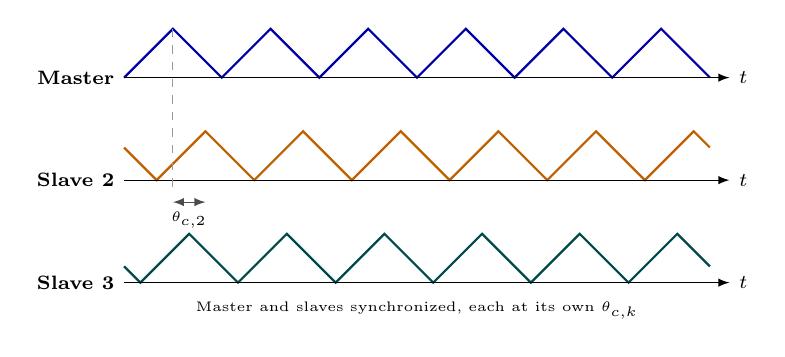
\begin{tikzpicture}[font=\scriptsize,x=6.2mm,y=6.2mm,>=latex]
% ---- Master carrier (blue), baseline y=0 ----
\draw[blue!65!black,thick]
  (0,0)--(1,1)--(2,0)--(3,1)--(4,0)--(5,1)--(6,0)
  --(7,1)--(8,0)--(9,1)--(10,0)--(11,1)--(12,0);
\draw[->] (0,0) -- (12.4,0) node[right] {$t$};
\node[left] at (0,0) {\textbf{Master}};
% ---- Slave 2 (orange), phase offset theta_c,2, baseline y=-2.1 ----
\draw[orange!75!black,thick]
  (0,-2.1+0.667)--(0.667,-2.1)--(1.667,-2.1+1)--(2.667,-2.1)
  --(3.667,-2.1+1)--(4.667,-2.1)--(5.667,-2.1+1)--(6.667,-2.1)
  --(7.667,-2.1+1)--(8.667,-2.1)--(9.667,-2.1+1)--(10.667,-2.1)
  --(11.667,-2.1+1)--(12,-2.1+0.667);
\draw[->] (0,-2.1) -- (12.4,-2.1) node[right] {$t$};
\node[left] at (0,-2.1) {\textbf{Slave 2}};
% ---- Slave 3 (teal), phase offset theta_c,3, baseline y=-4.2 ----
\draw[teal!58!black,thick]
  (0,-4.2+0.333)--(0.333,-4.2)--(1.333,-4.2+1)--(2.333,-4.2)
  --(3.333,-4.2+1)--(4.333,-4.2)--(5.333,-4.2+1)--(6.333,-4.2)
  --(7.333,-4.2+1)--(8.333,-4.2)--(9.333,-4.2+1)--(10.333,-4.2)
  --(11.333,-4.2+1)--(12,-4.2+0.333);
\draw[->] (0,-4.2) -- (12.4,-4.2) node[right] {$t$};
\node[left] at (0,-4.2) {\textbf{Slave 3}};
\node[below,font=\tiny] at (6,-4.4)
  {Master and slaves synchronized, each at its own $\theta_{c,k}$};
% ---- theta_c,2 annotation between master and slave-2 peaks ----
\draw[dashed,black!40,thin] (1,1) -- (1,-2.4);
\draw[<->,black!70] (1,-2.55) -- (1.667,-2.55);
\node[below,font=\tiny] at (1.33,-2.55) {$\theta_{c,2}$};
\end{tikzpicture}
\caption{Master/slave carrier synchronization for a representative
$N=3$ example: each slave's carrier is offset from the master by its
own phase $\theta_{c,k}$ \eqref{eq:carrier_phase}.}
\label{fig:carrier_sync_mechanism}
\end{figure}


\subsection{DC-Link Ripple Reduction and Battery-Side Current}

DC-link current ripple accelerates battery aging and is itself a
design objective. Lower-voltage cell switches typically enable a
higher switching frequency for a given loss budget, reducing the
required per-cell capacitance and battery-side ripple relative to a
single high-voltage bridge; carrier-phase interleaving reduces this
ripple further still.

The cell's dc-side current follows from convolving each phase's
switching-function spectrum with its current spectrum and summing over
the three phases,
\begin{equation}
I_{\mathrm{conv},x,k}=\tfrac12\left(S_{x,k}\otimes I_{x,k}\right).
\label{eq:conv_current_spectrum}
\end{equation}

For a single cell, every carrier harmonic $m$ contributes sidebands at
$n=\pm6p-3$ ($m$ odd) or $n=\pm6p$ ($m$ even), for integer $p$. With
uniform interleaving $\theta_{c,k}=2\pi k/N$, summing the $N$ cells'
converter currents shows that only carrier harmonics that are
themselves multiples of $N$ survive ($m=pN$ for even $N$, $m=2pN$ for
odd $N$), each retaining the same sideband structure
\cite{Jin2014Control}.


Translating this converter-current spectrum into the dc-link current
actually shared by the series stack requires the SPB equivalent
circuit of Section~\ref{sec:dclink_balancing},
\begin{equation}
L\frac{di_{\mathrm{dc}}}{dt}=E-Ri_{\mathrm{dc}}-\sum_kv_{\mathrm{conv},k},
\qquad
C_k\frac{dv_{\mathrm{conv},k}}{dt}=i_{\mathrm{dc}}-i_{\mathrm{conv},k},
\label{eq:dclink_ode}
\end{equation}
giving a closed-form transfer function between the summed
converter-current spectrum and the resulting dc-bus current
\cite{Jin2014Control},
\begin{equation}
I_{\mathrm{dc}}(\omega)=\frac{\sum_{k=1}^{N}I_{\mathrm{conv},k}(\omega)}
{N-\omega^2LC+j\omega CR}.
\label{eq:battery_current_tf}
\end{equation}
Because the residual dc-link ripple is dominated by the lowest
surviving harmonic, $m=N$, evaluating
\eqref{eq:battery_current_tf} there gives an approximate ripple
estimate,
\begin{equation}
\Delta i_{\mathrm{dc}}\approx\frac{\left|\sum_{k=1}^{N}
I_{\mathrm{conv},k}(2\pi Nf_{sw})\right|}
{\left|N-(2\pi Nf_{sw})^2LC+j2\pi Nf_{sw}CR\right|}.
\label{eq:dclink_ripple_estimate}
\end{equation}

Because the surviving harmonic sits at $N$ times the per-cell
switching frequency, both the removal of the uncancelled low-order
sidebands and the higher-frequency $LC$ attenuation act in the same
direction. Fig.~\ref{fig:dclink_ripple_interleaving} illustrates this
by simulation for a representative $N=3$ case.

\begin{figure}[!t]
\centering
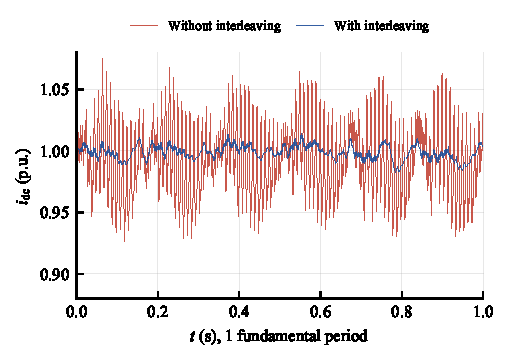
\includegraphics[width=\columnwidth]{Figures/fig_dclink_ripple.pdf}
\caption{Coupled circuit simulation of the shared series dc-link
current $i_{\mathrm{dc}}(t)$ for $N=3$ SPB cells ($M=0.85$,
$f_1=1$~Hz, $f_{sw}=100$~Hz), without (red) and with (blue) carrier
interleaving between submodules \eqref{eq:carrier_phase}. Both traces
share the same dc average; interleaving reduces the peak-to-peak
ripple by roughly $4$--$5\times$, consistent with
\eqref{eq:dclink_ripple_estimate}. Computed simulation result, not
measured hardware data.}
\label{fig:dclink_ripple_interleaving}
\end{figure}

This simulation lumps the battery-to-stack bus inductance but treats
each cell's own connection to that bus as ideal. In a physically
distributed implementation, each cell instead reaches the shared dc
path through its own bus-bar and connector loop, whose parasitic
inductance couples back into the cancellation mechanism itself: Wang
\textit{et al.} \cite{Wang2015GaNIMMD} found that a series-connected
GaN IMMD required careful capacitor selection and tight layout to
preserve the benefit of interleaving, and an earlier characterization
of an interleaved series-connected drive found that parasitic loop
inductance could make the interleaved ripple larger than the
non-interleaved case \cite{Wang2015ThesisDVB}. The reduction in
Fig.~\ref{fig:dclink_ripple_interleaving} should therefore be read as
an upper bound, with the achievable benefit set by layout, capacitor
selection, and switching frequency rather than by carrier phasing
alone.

\subsection{Machine Harmonics, Voltage Utilization, and Switching Loss}

The optimum carrier displacement is nonetheless
not universal: it depends on cell count, modulation index, power
factor, winding displacement, and the specific quantity being
minimized, so carrier coordination should be viewed as one design
variable within a larger converter--machine modulation problem.

SPB-specific studies show that inter-cell modulation affects both semiconductor losses and
dc-link-current harmonics \cite{Jin2017Modulation}, and related
modular and multiphase drives demonstrate simultaneous reduction of
dc-link and machine current ripple
\cite{Verkroost2021Ripple,DeMarcos2025InterleavedPWM,Wang2025HybridPWM}.

The multiphase machine makes the harmonic problem substantially more
involved than in a conventional three-phase drive: nonfundamental
voltage components can excite additional harmonic subspaces with low
impedance, producing copper loss and torque ripple even when
fundamental current control is fully satisfactory. Recent
integrated-modular-drive studies accordingly move toward interleaved
and discontinuous PWM techniques tailored to this multiphase
current-ripple problem
\cite{Hopkins2019DCLinkRipple,Mohamed2020DCLinkSizing,Alosa2019ModularRipple}.

At high speed, modulation must also maximize voltage utilization,
because each winding group is supplied only from its local cell
voltage $V_{\mathrm{dc},k}$, as constrained by
\eqref{eq:spb_machine_voltage_limit} -- an objective that grows more
important as $N$ increases and $V_{\mathrm{dc},k}$ falls accordingly.
Optimized vector selection for dual-three-phase traction machines has
demonstrated the possibility of extending the high-modulation region
while simultaneously suppressing unwanted subspace currents
\cite{Chen2026HighModulationDTP}.

Switching loss introduces an opposing objective. DPWM and hybrid
strategies reduce the number of transitions by clamping selected
phases or by redistributing high-frequency switching among converter
modules. Related open-end-winding (OEW) work demonstrates that
coordinated modulation can reduce switching loss and unwanted
zero-sequence current simultaneously \cite{Yang2026HybridOEW,
Lee2026AlternatingDPWM}; although its dc architecture differs, the
underlying principle of distributing switching activity among several
inverter modules is directly transferable to SPB.

\subsection{Coupling to Balancing and Common-Mode Objectives}

Modulation also sets the achievable authority for two further
objectives that are developed as dedicated topics later in this paper:
dc-link voltage balancing (Section~\ref{sec:dclink_balancing}), where
differential winding-group power must be realizable through modulation
without violating local voltage and current limits
\cite{Verkroost2024PowerDistribution,Wu2020ActiveBalancing,
Mocevic2024GateDelay}; and common-mode voltage (Section~\ref{sec:common_mode}),
where redundant voltage vectors or coordinated zero-sequence terms can
reduce frame excitation \cite{Sun2025CMVMPC,Zheng2025MultiObjectivePWM,
Chen2020EMCIntegrated}. 
The key SPB modulation question is therefore
not which conventional PWM method performs best in isolation, but how
switching decisions should be coordinated across cells to jointly
manage ripple, loss, balancing, and common-mode objectives over the
full operating map.

% ============================================================================
\section{Common-Mode Voltage Effects}
\label{sec:common_mode}
% ============================================================================

In any converter-fed ac machine, the non-zero average of the three
phase-leg pole voltages produced by PWM switching gives rise to a
common-mode voltage (CMV) that excites parasitic capacitive paths
between winding, frame, shaft, and bearings. This mechanism is well
characterized for a converter with a single machine port whose voltage
scaling is produced internally, such as the flying-capacitor
multilevel converter, for which an analytical CM-EMI model referenced
to one dc-link potential exists \cite{Giardine2025FCMLEMI}. SPB does
not fit this picture: because its $N$ cells are connected in series on
the dc side (Section~\ref{sec:operating_principle}) while each feeds
an electrically separate winding group, cell $k$'s local dc rails are
displaced from the overall dc-bus reference by an amount that depends
on its position in the stack.

\subsection{Series-Stack Origin of Common-Mode Excitation}

Taking cell 1's negative dc rail as the reference, with cell $k$'s
negative rail coinciding with cell $(k-1)$'s positive rail, the
absolute offset of cell $k$ is

\begin{equation}
V_{-,k}=\sum_{j=1}^{k-1}V_{\mathrm{dc},j}
\approx(k-1)\frac{V_{\mathrm{dc}}}{N},
\label{eq:spb_cm_offset}
\end{equation}

using the voltage-partitioning relation \eqref{eq:spb_voltage_sum}. The
common-mode potential seen by winding group $k$ is then

\begin{equation}
v_{\mathrm{cm},k}^{\mathrm{abs}}(t)=
V_{-,k}+\frac{1}{3}\left(v_{aN_k}+v_{bN_k}+v_{cN_k}\right),
\label{eq:spb_cm_local}
\end{equation}

where $v_{aN_k},v_{bN_k},v_{cN_k}$ are cell $k$'s pole voltages
referenced to its own negative rail $N_k$. The second term is the
conventional switching-induced CMV already addressed by zero-sequence
injection and vector-redundancy modulation
(Section~\ref{sec:modulation}); the first term, $V_{-,k}$, is specific
to SPB, set by the cell's stack position and by the instantaneous
voltage-sharing state (Section~\ref{sec:dclink_balancing}), not by
modulation alone.

Fig.~\ref{fig:spb_cm_stack} illustrates the resulting structure:
increasing absolute potential offset with stack position, together
with representative CM current paths coupling each winding group to
the shared frame and chassis ground through parasitic capacitance.
Because the cells and their winding groups are physically close
together in the integrated implementations of
Section~\ref{sec:machine_requirements}, these paths are short and the
coupling between cells is direct rather than mediated by long cabling.
Physically integrated motor-drive assemblies show that common-mode
current can resonate through exactly this kind of parasitic loop, and
that the resonance is not adequately predicted by a single-source CM
model \cite{Zhong2025CMResonance,Chen2020EMCIntegrated} -- extending
such modeling to a multi-port structure with $N$ distinct dc offsets
is, to the authors' knowledge, not yet available for SPB specifically.

\begin{figure}[!t]
\centering
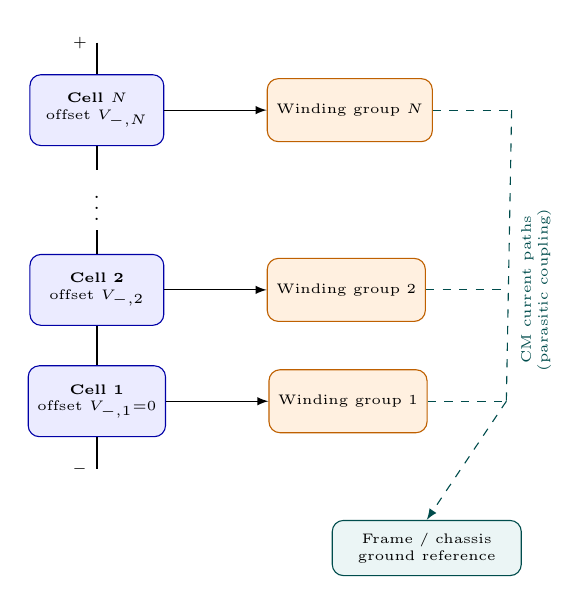
\begin{tikzpicture}[font=\scriptsize,>=latex,node distance=5mm]
\tikzstyle{cell}=[draw=blue!65!black,rounded corners,minimum width=17mm,
  minimum height=9mm,align=center,fill=blue!8,font=\tiny]
\tikzstyle{wind}=[draw=orange!75!black,rounded corners,minimum width=19mm,
  minimum height=8mm,align=center,fill=orange!12,font=\tiny]
\tikzstyle{gndbox}=[draw=teal!60!black,rounded corners,minimum width=24mm,
  minimum height=7mm,align=center,fill=teal!8,font=\tiny]

\node[cell] (cN) {\textbf{Cell $N$}\\ offset $V_{-,N}$};
\node[font=\scriptsize,below=3mm of cN] (dots) {$\vdots$};
\node[cell,below=3mm of dots] (c2) {\textbf{Cell 2}\\ offset $V_{-,2}$};
\node[cell,below=5mm of c2] (c1) {\textbf{Cell 1}\\ offset $V_{-,1}{=}0$};

\node[wind,right=13mm of cN] (wN) {Winding group $N$};
\node[wind,right=13mm of c2] (w2) {Winding group 2};
\node[wind,right=13mm of c1] (w1) {Winding group 1};

\draw[->] (cN.east) -- (wN.west);
\draw[->] (c2.east) -- (w2.west);
\draw[->] (c1.east) -- (w1.west);

\coordinate (topdc) at ([yshift=4mm]cN.north);
\draw[thick] (topdc) -- (cN.north);
\node[font=\tiny,left] at (topdc) {$+$};
\draw[thick] (cN.south) -- (dots.north);
\draw[thick] (dots.south) -- (c2.north);
\draw[thick] (c2.south) -- (c1.north);
\coordinate (botdc) at ([yshift=-4mm]c1.south);
\draw[thick] (c1.south) -- (botdc);
\node[font=\tiny,left] at (botdc) {$-$};

\node[gndbox,below=11mm of w1,xshift=10mm] (gnd)
  {Frame / chassis\\ ground reference};

\coordinate (busN) at ([xshift=10mm]wN.east);
\coordinate (bus2) at ([xshift=10mm]w2.east);
\coordinate (bus1) at ([xshift=10mm]w1.east);

\draw[teal!60!black,dashed] (wN.east) -- (busN);
\draw[teal!60!black,dashed] (w2.east) -- (bus2);
\draw[teal!60!black,dashed] (w1.east) -- (bus1);
\draw[teal!60!black,dashed] (busN) -- (bus1);
\draw[teal!60!black,dashed,->] (bus1) -- (gnd.north);
\node[font=\tiny,teal!60!black,align=center,rotate=90] at ([xshift=4mm]bus2)
  {CM current paths\\(parasitic coupling)};
\end{tikzpicture}
\caption{Simplified SPB series-stack structure: absolute potential
offset per cell \eqref{eq:spb_cm_offset} and representative CM current
paths (dashed) to the shared frame/chassis ground through parasitic
capacitance.}
\label{fig:spb_cm_stack}
\end{figure}

\subsection{Carrier Synchronization for CMV Cancellation}

Beyond the stack-offset mechanism above, synchronizing each cell's PWM
waveform relative to the others is a way to actively cancel the
switching-induced component of CMV. We illustrate the principle for
the $N=2$ case, where the cancellation condition has a simple closed
form; the same synchronization idea extends to larger stacks built
from matched cell pairs, though a general $N$-cell synchronization law
has not yet been derived for SPB.

If cell 2 is driven with the logical inverse of cell 1's gate
commands, and cell 2's winding set is wired with reversed winding
sense so that both cells still generate torque in the same direction,
the two cells' individually switched CMVs become approximately equal
and opposite, $v_{\mathrm{cm},1}(t)\approx-v_{\mathrm{cm},2}(t)$, and
the total CMV seen by the machine,
\begin{equation}
v_{\mathrm{cm,tot}}(t)=\frac{v_{\mathrm{cm},1}(t)+v_{\mathrm{cm},2}(t)}{2},
\label{eq:spb_cm_cancellation}
\end{equation}
cancels toward zero instead of adding constructively. This
balanced-cancellation principle was first demonstrated for a
dual-winding-set machine driven by a balanced inverter pair on a
single, non-series-stacked machine \cite{Han2018CMCancellation}, and
was later applied to a genuine two-cell series-stacked (2L-SSC) SPB
inverter \cite{Rohner2024GaN}; as with interleaved GaN IMMDs, the
achievable reduction is ultimately limited by layout parasitics and
local dc-link capacitor design \cite{Wang2015GaNIMMD}.

This cancellation assumes perfectly matched, simultaneous switching
transitions between the two cells: a propagation-delay mismatch (e.g.,
from PCB layout or driver differences) reintroduces a residual CM
spike, of duration equal to the delay, at every misaligned transition,
and unequal power sharing during dc-link balancing similarly degrades
the cancellation, both shown quantitatively in
\cite{Rohner2024GaN,Han2018CMCancellation}. The mechanism is specific
to $N=2$, or to a stack of matched cell pairs, so it should be read as
a valuable special-case mitigation rather than a general solution to
the stack-offset problem above. Fig.~\ref{fig:spb_cm_cancellation}
simulates this cancellation directly from switching-function
waveforms, including its effect on the resulting bearing/ground
current.

\begin{figure}[!t]
\centering
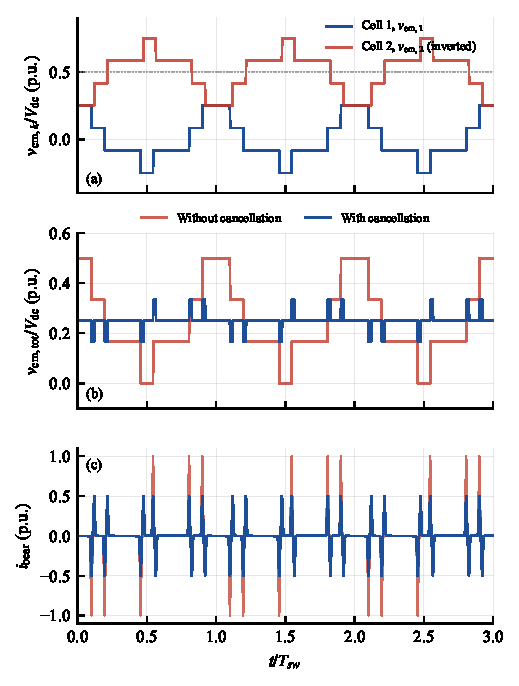
\includegraphics[width=\columnwidth]{Figures/fig_cm_cancellation.pdf}
\caption{Switching-function simulation of $N=2$ SPB common-mode
cancellation ($M=0.85$, $\cos\varphi\approx0.94$), all quantities in
per unit, with cell~2 driven by the logically inverted gate commands of
cell~1 plus a propagation delay $t_d=0.02\,T_{sw}$. (a)~Each cell's
absolute CM voltage $v_{\mathrm{cm},k}^{\mathrm{abs}}$, combining the
stack offset $V_{-,k}$~\eqref{eq:spb_cm_offset} with its local
switching term. (b)~Total CM voltage
$v_{\mathrm{cm,tot}}(t)$~\eqref{eq:spb_cm_cancellation}: cancellation
removes the switching ripple, leaving only delay-induced residual
spikes on the same stack-offset average. (c)~Resulting bearing/ground
current $i_{\mathrm{bear}}=C\,dv_{\mathrm{cm,tot}}/dt$, normalized to
the without-cancellation peak. Computed simulation result, not
measured hardware data.}
\label{fig:spb_cm_cancellation}
\end{figure}

\subsection{Physical Consequences and Mitigation}

CMV-driven bearing current is a documented failure mechanism in
inverter-fed machines generally, arising from capacitive coupling
through the air gap and discharge events once the bearing lubricant
film breaks down \cite{Lee2025BearingCurrent}, and can be identified
with dedicated non-intrusive current-measurement techniques
\cite{Li2025BearingMeasurement}. In SPB, this mechanism acts at each of
the $N$ winding groups individually; because
\eqref{eq:spb_cm_offset}--\eqref{eq:spb_cm_local} gives each group a
different absolute CM reference, the resulting bearing- and
shaft-voltage stress is not necessarily uniform across the stack, and
whether it is dominated by the highest-offset cell, by all cells
combined, or by resonant interaction between cells remains open.
Shaft-voltage cancellation circuits developed for conventional drives
\cite{Xie2026ShaftCM} are a plausible mitigation candidate but have not
been demonstrated for a series-stacked, multi-port machine.

The same switching events also produce fast $dv/dt$ transitions at the
winding terminals, stressing turn-to-turn and phase-to-frame
insulation independently of the CM current path. WBG devices, already
motivated for SPB by their favorable scaling at reduced blocking
voltage (Section~\ref{sec:semiconductor_scaling}), shorten rise time
and increase overshoot, and have been shown to accelerate insulation
aging and partial-discharge activity in hairpin and other
traction-machine windings \cite{KholghKhiz2025HairpinWBG,
Gulec2025PDImpulse,Seri2025ATFPDIV}; diagnostic methods exist to assess
the resulting insulation condition \cite{Kim2025HairpinFRA}, within the
broader set of insulation technologies for transport-electrification
machines \cite{Martinez2025TransportInsulation}. In SPB, this stress is
superimposed on the stack-position-dependent offset of
\eqref{eq:spb_cm_offset}, so insulation coordination must account for
both the local switching transition and the cell's absolute stack
position, consistent with the challenge identified qualitatively in
Section~\ref{sec:machine_requirements}.

Mitigation therefore has to act at more than one level. Active EMI
filtering can attenuate common-mode current at the converter terminals
without relying on machine or bearing hardware
\cite{Ihsan2025ActiveEMI}, and cancellation circuits can target shaft
voltage directly \cite{Xie2026ShaftCM}. At the modulation level,
Section~\ref{sec:modulation} showed that zero-sequence injection and
redundant-vector selection reduce CMV excitation
\cite{Sun2025CMVMPC,Zheng2025MultiObjectivePWM}, but the carrier-phase
displacement used there to interleave switching harmonics for ripple
reduction, \eqref{eq:carrier_phase}, is chosen to cancel a selected
ripple harmonic and is not simultaneously optimized for common-mode
excitation. Because SPB's CM problem additionally depends on the fixed
stack offset $V_{-,k}$, which carrier phasing cannot change, an
interleaving choice that minimizes dc-link or stator ripple need not
minimize aggregate common-mode excitation, and vice versa -- a genuine
SPB-specific design tension that future studies should address by
extending the multi-objective modulation problem of
Section~\ref{sec:modulation} to common-mode and insulation-stress
metrics evaluated across the full stack.

% ============================================================================
\section{DC-Link Dynamics, Stability, and Voltage Balancing}
\label{sec:dclink_balancing}
% ============================================================================

The shared dc current and independently controllable winding-group
powers (Section~\ref{sec:operating_principle}) make the local
capacitors coupled energy-storage states whose voltages are not
guaranteed to remain equal
\cite{Nikouie2015Stability,Nikouie2017Stability}, a conclusion also
reached independently for a series-connected multilevel motor drive,
where distributed closed-loop current control alone was shown to leave
the module voltages inherently unstable without dedicated balancing
action \cite{Wang2015ThesisDVB}.

For cell $k$,
\begin{equation}
C_kV_{\mathrm{dc},k}\frac{dV_{\mathrm{dc},k}}{dt}
=
V_{\mathrm{dc},k}i_{\mathrm{dc}}
-p_{\mathrm{ac},k}
-p_{\mathrm{loss},k}.
\label{eq:spb_voltage_dynamic}
\end{equation}
This captures the essential balancing mechanism: dc input power
depends directly on local cell voltage because the series current is
common, while output power is set independently by the corresponding
winding group's controller.

For analysis, define
\begin{equation}
\widetilde V_k=
V_{\mathrm{dc},k}
-\frac{1}{N}\sum_{j=1}^{N}V_{\mathrm{dc},j}.
\label{eq:cell_voltage_deviation}
\end{equation}
A simplified differential-mode model around a balanced point is
\begin{equation}
CV_0\frac{d\widetilde V_k}{dt}
\approx
I_{\mathrm{dc},0}\widetilde V_k-\Delta P_k.
\label{eq:linearized_balance_dynamic}
\end{equation}
In motoring operation ($I_{\mathrm{dc},0}>0$), a positive cell-voltage
perturbation increases that cell's dc input power and can reinforce the
deviation if the ac-side power is unchanged; in regeneration the
feedback sign reverses. This simplified picture is consistent with the
detailed SPB stability analyses in
\cite{Nikouie2015Stability,Nikouie2017Stability} and with recent work
on related series-connected multiphase drives
\cite{Ni2025SeriesDCLinkStability}.

Reference~\cite{Nikouie2017Stability} derives this instability directly
from the full nonlinear constant-power-load model, without the
small-signal approximation of \eqref{eq:linearized_balance_dynamic}:
with $L_b\,di_{\mathrm{dc}}/dt=E_b-R_bi_{\mathrm{dc}}-\sum_kV_{\mathrm{dc},k}$
and $C_k\,dV_{\mathrm{dc},k}/dt=i_{\mathrm{dc}}-P_k/V_{\mathrm{dc},k}$, the
open-loop characteristic polynomial has $N-1$ real, strictly positive
eigenvalues in motoring operation ($P_k>0$) for any $N>1$ -- the series
stack is provably unstable without a balancing controller, regardless
of parameter choice. Fig.~\ref{fig:spb_balancing_dynamics} integrates
this exact nonlinear model using the real experimental parameters of
\cite{Nikouie2017Stability} ($L_b=8\,\mu\text{H}$, $R_b=0.35\,\Omega$,
$C=100\,\mu\text{F}$ per cell): without balancing, a small initial
imbalance collapses one cell's voltage within milliseconds, while the
proportional balancing law of \cite{Nikouie2017Stability} (their
``controller alternative I'') drives the same imbalance back to zero on
a comparable timescale.

\begin{figure}[!t]
\centering
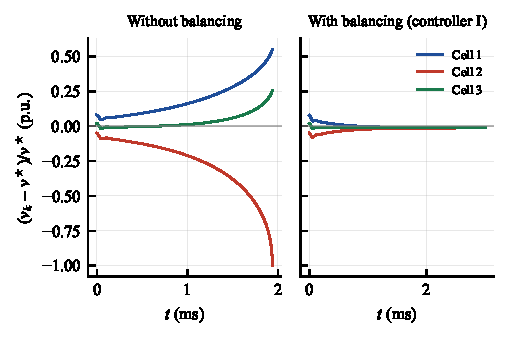
\includegraphics[width=\columnwidth]{Figures/fig_dclink_balancing.pdf}
\caption{Nonlinear dc-link voltage-sharing simulation for $N=3$ cells,
without (left) and with (right) the balancing controller of
\cite{Nikouie2017Stability}. Computed simulation result, not measured
hardware data.}
\label{fig:spb_balancing_dynamics}
\end{figure}

The multiple winding groups provide a natural actuator for controlling
internal capacitor energy. The cell power reference can be decomposed
as
\begin{equation}
P_k^\star=\frac{P^\star}{N}+\Delta P_k,
\qquad
\sum_{k=1}^{N}\Delta P_k=0,
\label{eq:balancing_power}
\end{equation}
so differential power redistributes internal energy without changing
the requested total machine power. In practice $\Delta P_k$ is limited
by phase-current margin, winding voltage, torque-ripple constraints,
and thermal state, so balancing authority is operating-point
dependent.

Three main SPB balancing approaches can be identified. Centralized
active balancing uses measured capacitor voltages to generate
differential current or power commands
\cite{Nikouie2015Stability,Nikouie2017Stability}. Common-duty-ratio
(CDR) control applies common modulation commands and can obtain stable
voltage sharing from the natural converter--machine dynamics for the
investigated induction-machine system \cite{Mocevic2023CDR}, though
practical timing mismatch remains important
\cite{Mocevic2024GateDelay}. Distributed multi-agent control uses local
measurements and neighbour communication, and has been demonstrated
for voltage balancing, power sharing, and reconfiguration
\cite{Verkroost2024VoltageBalance,Verkroost2024PowerDistribution,
Verkroost2024Reconfiguration}, comparable to the local droop laws that
coordinate power sharing across modules in the speed-droop framework of
Galassini \textit{et al.} \cite{Galassini2016ModularSpeedDroop}.
Table~\ref{fig:spb_balancing_taxonomy} summarizes these approaches and
their principal considerations.

\begin{table}[!t]
\centering
\caption{Principal SPB dc-link balancing approaches and their main
considerations.}
\label{fig:spb_balancing_taxonomy}
\renewcommand{\arraystretch}{1.15}
\setlength{\tabcolsep}{3pt}
\footnotesize
\begin{tabular}{p{1.6cm}p{2.9cm}p{2.6cm}}
\hline
\textbf{Approach} & \textbf{Mechanism} & \textbf{Key consideration}\\
\hline
Centralized & Differential current/power commands
\cite{Nikouie2015Stability,Nikouie2017Stability} &
Direct authority; global sensing and coordination\\
CDR & Common modulation, natural coupled dynamics
\cite{Mocevic2023CDR,Mocevic2024GateDelay} &
Low overhead; symmetry- and timing-sensitive\\
Distributed & Local agents, neighbour communication
\cite{Verkroost2024VoltageBalance,Verkroost2024PowerDistribution,
Verkroost2024Reconfiguration} &
Scalable; requires communication and synchronization\\
\hline
\end{tabular}
\end{table}

For automotive operation, balancing must remain effective through
torque transients, field weakening, parameter mismatch, and module
reconfiguration: voltage-sensor offset, communication latency,
propagation delay, and the available differential current/power margin
can determine the usable cell-voltage margin and, consequently, the
semiconductor rating.

This underscores the section's central point: dc-link stability
belongs to the complete converter--machine--control system, not the
power stage alone.

% ============================================================================
\section{Semiconductor Technology and Cell-Count Scaling}
\label{sec:semiconductor_scaling}
% ============================================================================

Semiconductor voltage scaling (Section~\ref{sec:semiconductor_limitations})
and the voltage-versus-component-count tradeoff established in
Section~\ref{sec:operating_principle} are quantified here at the
cell-count level. In an $N$-cell SPB, the dc-link voltage is
distributed among the series-connected converter cells, allowing the
use of lower-voltage semiconductor classes as $N$ increases.

The device rating must be selected from the maximum expected blocking
stress, not the nominal voltage division alone:
\begin{equation}
V_{\mathrm{rated}}
\geq
k_{\mathrm{rel}}
\left(
\frac{V_{\mathrm{dc,max}}}{N}
+\Delta V_{\mathrm{imb}}^{\max}
+\Delta V_{\mathrm{sw}}^{\max}
\right),
\label{eq:semiconductor_rating}
\end{equation}
where $\Delta V_{\mathrm{imb}}^{\max}$ denotes the maximum cell-voltage
imbalance, $\Delta V_{\mathrm{sw}}^{\max}$ the commutation overshoot,
and $k_{\mathrm{rel}}$ the selected reliability margin. Cell count is
therefore linked to discrete commercial voltage classes rather than to
a continuous semiconductor-scaling law.

As introduced in Section~\ref{sec:semiconductor_limitations}, SiC
currently provides the most direct route for high-voltage traction,
whereas GaN becomes increasingly attractive once the architecture
reduces the per-device voltage enough to access lower-voltage classes
with favorable conduction and switching characteristics
\cite{WBGTractionReview2025,Rohner2024GaN,Ebrahimian2025GaNIMMD}.

The resulting discrete design transitions are summarized and
visualized directly in Fig.~\ref{fig:cell_count_scaling}. For a
1200-V dc link, $N=2$ gives a nominal cell voltage of 600~V and
therefore leaves limited transient margin for a 650-V device.
Increasing the cell count to $N=3$ reduces the nominal cell voltage
to 400~V and provides a substantially more practical operating region
for the 650-V class. Further increases in $N$ give access to
progressively lower-voltage device families, as labeled directly on
Fig.~\ref{fig:cell_count_scaling}. The potential semiconductor benefit
is therefore nonlinear because a small change in $N$ can open a new
commercial voltage class, whereas the active-switch count grows
approximately linearly, as plotted directly from these design points
in Fig.~\ref{fig:cell_count_scaling}.

\begin{figure}[!t]
\centering
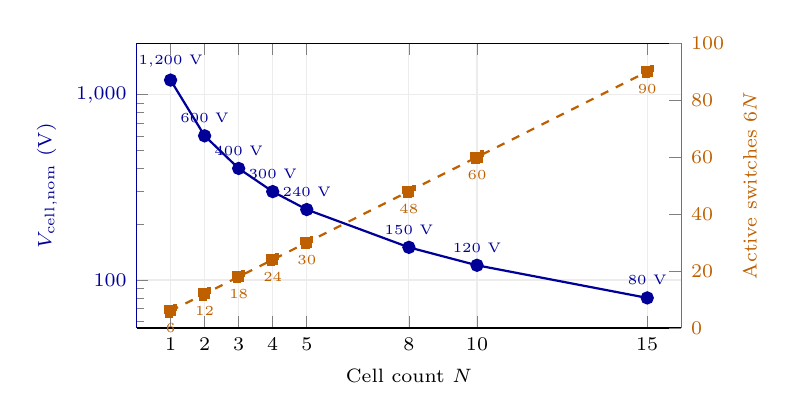
\begin{tikzpicture}
\begin{axis}[
    width=8.5cm,
    height=52mm,
    font=\scriptsize,
    xlabel={Cell count $N$},
    ylabel={$V_{\mathrm{cell,nom}}$ (V)},
    ymode=log,
    log ticks with fixed point,
    xmin=0,xmax=16,
    ymin=55,ymax=1900,
    xtick={1,2,3,4,5,8,10,15},
    axis y line*=left,
    y axis line style={draw=blue!60!black},
    tick label style={font=\scriptsize},
    yticklabel style={blue!60!black},
    xlabel style={font=\scriptsize},
    ylabel style={font=\scriptsize,blue!60!black},
    grid=major,
    grid style={gray!15},
]
\addplot[mark=*,thick,blue!60!black,
    point meta=explicit,
    nodes near coords={\pgfmathprintnumber{\pgfplotspointmeta}~V},
    every node near coord/.append style={font=\tiny,blue!60!black,anchor=south,yshift=1pt}]
    coordinates {
(1,1200)[1200](2,600)[600](3,400)[400](4,300)[300](5,240)[240]
(8,150)[150](10,120)[120](15,80)[80]};
\end{axis}
\begin{axis}[
    width=8.5cm,
    height=52mm,
    font=\scriptsize,
    xmin=0,xmax=16,
    ymin=0,ymax=100,
    xtick={1,2,3,4,5,8,10,15},
    axis x line=none,
    axis y line*=right,
    y axis line style={draw=orange!75!black},
    ylabel={Active switches $6N$},
    tick label style={font=\scriptsize},
    yticklabel style={orange!75!black},
    ylabel style={font=\scriptsize,orange!75!black},
]
\addplot[mark=square*,thick,dashed,orange!75!black,
    point meta=y,
    nodes near coords={\pgfmathprintnumber{\pgfplotspointmeta}},
    every node near coord/.append style={font=\tiny,orange!75!black,anchor=north,yshift=-1pt}]
    coordinates {
(1,6)(2,12)(3,18)(4,24)(5,30)(8,48)(10,60)(15,90)};
\end{axis}
\end{tikzpicture}
\caption{Cell-count scaling for a 1200-V dc link: nominal cell voltage
$V_{\mathrm{cell,nom}}=V_{\mathrm{dc}}/N$ (solid markers, left log
axis) and active-switch count $6N$ (dashed markers, right linear
axis) versus cell count $N$; every marker is labeled directly with
its exact value ($N=1$: 1200~V, 6; $N=2$: 600~V, 12; $N=3$: 400~V,
18; $N=4$: 300~V, 24; $N=5$: 240~V, 30; $N=8$: 150~V, 48; $N=10$:
120~V, 60; $N=15$: 80~V, 90). Increasing $N$ opens progressively lower
commercial semiconductor voltage classes (e.g., 1700--2000-V SiC at
$N=1$, 650-V GaN/SiC at $N=3$, 100-V GaN/MOSFET class at $N=15$) while
the active-switch count grows linearly as $6N$.}
\label{fig:cell_count_scaling}
\end{figure}

\subsection{Commercial-Device Screening}

Access to a lower voltage class does not by itself imply a superior
converter: the comparison must be based on commercial devices and
their conduction, switching, current, thermal, and packaging
constraints.

For nonlinear output capacitance, the stored energy
\begin{equation}
E_{\mathrm{oss}}(V)
=
\int_{0}^{V}
vC_{\mathrm{oss}}(v)\,dv
\label{eq:eoss_integral}
\end{equation}
is more informative than a single tabulated $C_{\mathrm{oss}}$ value.
Depending on the commutation process, some or all of this stored energy
can contribute to switching loss. Similarly, simple screening metrics
such as $R_{\mathrm{DS(on)}}C_{\mathrm{oss}}$ or
$R_{\mathrm{DS(on)}}Q_g$ are useful for identifying candidate devices,
but are insufficient for the final architecture comparison.

The principal device quantities required for SPB cell-count screening,
and their primary role in the comparison, are: $R_{\mathrm{DS(on)}}(T)$,
which sets the die-area or parallel-device requirement;
$E_{\mathrm{oss}}(V)$, which sets the large-signal switching penalty;
$E_{\mathrm{on/off}}(V,I,T)$, which forms the operating-point
switching-loss model; gate charge $Q_g$ and $Q_{gd}$, which govern
driver sizing and auxiliary loss; continuous current capability
$I_{\mathrm{cont}}$ and thermal resistance $R_\theta$, which govern
parallelization and cooling requirements; and package or loop
inductance $L_\sigma$, which sets the usable blocking-voltage margin
against $di/dt$-induced overshoot.

Current capability is particularly important because machine phase
current does not generally decrease in proportion to $1/N$
(Section~\ref{sec:operating_principle}). If the
derated current capability of one device is $I_{\mathrm{dev,der}}$, the
required number of parallel devices can be estimated as
\begin{equation}
n_p
=
\left\lceil
\frac{I_{\mathrm{sw,max}}}
     {I_{\mathrm{dev,der}}}
\right\rceil,
\qquad
N_{\mathrm{sw,tot}}
=
6Nn_p .
\label{eq:parallel_device_scaling}
\end{equation}
Thus, a lower-voltage device can offer an attractive device-level FOM
while still requiring substantial die area, package count, and
gate-drive/thermal interfaces. Recent high-current 650-V GaN
modules illustrate the importance of low-inductance packaging and
integrated gate driving when GaN is scaled toward traction-current
levels \cite{Zhu2024GaN150A,Rahman2025GaN300A}.

Fast switching further couples device selection to layout. The
commutation overshoot can be approximated by
\begin{equation}
\Delta V_{\mathrm{sw}}
\approx
L_{\sigma}\frac{di}{dt},
\label{eq:semiconductor_overshoot}
\end{equation}
so the benefit of reduced nominal cell voltage can be lost if package
and interconnect inductance consume a substantial fraction of the
available blocking margin. This is particularly relevant for GaN,
where high $di/dt$ places strong requirements on the commutation loop,
local decoupling, and gate-drive layout
\cite{Rahman2025GaN300A}.

GaN device selection also requires consideration of dynamic
$R_{\mathrm{DS(on)}}$, reverse conduction, gate reliability,
short-circuit capability, and thermal performance
\cite{Ajayan2025GaNReliability,Ajayan2025GaNFabrication}. These effects
do not negate the benefit of lower blocking voltage, but they prevent
room-temperature static $R_{\mathrm{DS(on)}}$ from being used as the
sole criterion for cell-count selection.

\subsection{Loss Scaling With Cell Count}

For one device, the dominant semiconductor losses can be represented
approximately as
\begin{equation}
P_{\mathrm{cond}}
\approx
I_{\mathrm{rms,sw}}^2
R_{\mathrm{DS(on)}}(T_j),
\label{eq:cond_loss_short}
\end{equation}
and
\begin{equation}
P_{\mathrm{sw}}
\approx
f_{\mathrm{sw}}
\left[
E_{\mathrm{on}}(V,I,T_j)
+
E_{\mathrm{off}}(V,I,T_j)
\right].
\label{eq:switching_loss_short}
\end{equation}

At converter level,
\begin{equation}
P_{\mathrm{semi}}(N)
=
\sum_{k=1}^{N}
\sum_{j=1}^{6n_p(N)}
\left(
P_{\mathrm{cond},k,j}
+
P_{\mathrm{sw},k,j}
+
P_{\mathrm{dt},k,j}
\right)
+
P_{\mathrm{gate}}(N).
\label{eq:complete_semiconductor_loss}
\end{equation}
The dependence on $N$ is therefore not linear. The number of active
devices increases with cell count, whereas
$R_{\mathrm{DS(on)}}$, switching energy, thermal impedance, and
parallel-device requirement can change abruptly when the design enters
a different semiconductor voltage class.

Consequently, SiC and GaN should be regarded as different regions of
the SPB design space rather than as a fixed technology ranking.
Low-cell-count architectures can favor high-voltage SiC because of its
mature voltage and current capability, whereas increasing $N$ can make
lower-voltage GaN attractive if the improvement in conduction,
switching, packaging, or passive-component performance compensates for
the additional converter modules.

Resolving the cell-count question therefore requires reading
Fig.~\ref{fig:cell_count_scaling} jointly with the screening
quantities above and the machine requirements of
Section~\ref{sec:machine_requirements}, rather than from any single
figure of merit.


% ============================================================================
\section{Fault Tolerance and Reconfiguration}
\label{sec:fault_reconfiguration}
% ============================================================================

SPB modularity provides structural redundancy because the converter and
machine are divided into repeated converter--winding modules. However,
fault tolerance is not automatic: because the dc ports are connected
in series, a failed cell can disturb or interrupt the complete dc
current path, a structural challenge demonstrated for SPB and for
other series-connected modular converters alike
\cite{Nikouie2016Fault,Zhang2014FaultToleranceFSCW,Gjerde2014SeriesFault}.
Early SPB work demonstrated post-fault operation under semiconductor
faults, establishing that repeated hardware must
be accompanied by appropriate safe states and control action
\cite{Nikouie2016Fault}. At the
machine level, a submodule short-circuit fault in a modular converter
feeding fractional-slot concentrated-winding PM machines was shown to
drive a fault current above rated current because of the strong
NdFeB rotor magnetization, risking machine overheating; reducing rotor
magnetization limits this fault current but also narrows the
constant-power-speed range, a design tradeoff specific to
fault-tolerant FSCW PM machines \cite{Zhang2014FaultToleranceFSCW}.
In the SPB machine designs of that study, post-fault short-circuit
current with NdFeB magnets exceeds the healthy-phase current, whereas
with ferrite magnets it stays below it, at the cost of becoming
visibly non-sinusoidal from magnetic coupling with the adjacent
healthy windings -- a concrete illustration that PM material selection
is itself a fault-tolerance design variable, not only a torque-density
one. Fault handling in other series-connected modular converters
further underscores that mitigation requires the control system to be
explicitly designed for module isolation \cite{Gjerde2014SeriesFault}.

The machine provides a second layer of redundancy. Healthy winding
groups can potentially redistribute current after phase or converter
faults, as demonstrated in recent multiphase and modular-drive studies
\cite{Tang2025SixPhaseFault,Zhang2025FaultTolerantMMD,
Du2026ModularPMSMFault}. In SPB, however, this machine-side redundancy
is useful only if the failed converter cell can be isolated or bypassed
without breaking the series dc path.

Building on the online reconfiguration capability introduced in
Section~\ref{sec:evolution} \cite{Verkroost2024Reconfiguration}, after
a faulted module is isolated the remaining active set $\mathcal{A}$
must satisfy
\begin{equation}
P^\star=\sum_{k\in\mathcal{A}}P_k^\star,
\label{eq:fault_power_redistribution}
\end{equation}
with torque derating if current, voltage, or thermal limits prevent full
redistribution. Reconfiguration can therefore provide both fault
isolation and an operating-range degree of freedom because the number
of active cells changes the voltage available to the remaining winding
groups. Isolating a cell also raises the voltage that each surviving
cell must share of the fixed dc-link voltage $V_{\mathrm{dc}}$
(\eqref{eq:spb_voltage_sum}, now divided among $|\mathcal{A}|<N$
active cells), which is an additional reason current or power
derating in \eqref{eq:fault_power_redistribution} may be needed after
a fault, as illustrated in Fig.~\ref{fig:spb_fault_response}.
Fig.~\ref{fig:spb_fault_locations} maps these fault locations
onto the SPB structure.

\begin{figure}[!t]
\centering
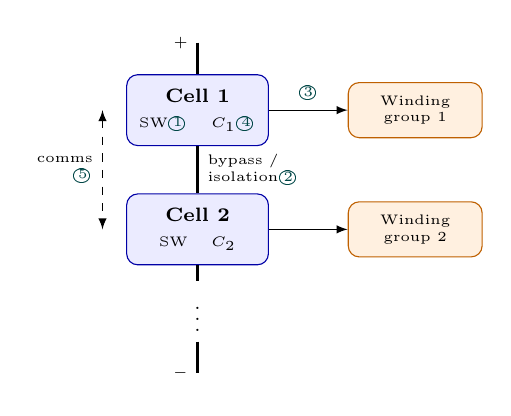
\begin{tikzpicture}[font=\scriptsize,>=latex,node distance=5mm]
\tikzstyle{cell}=[draw=blue!65!black,rounded corners,minimum width=18mm,
  minimum height=9mm,align=center,fill=blue!8]
\tikzstyle{wind}=[draw=orange!75!black,rounded corners,minimum width=17mm,
  minimum height=7mm,align=center,fill=orange!12,font=\tiny]

\node[cell] (c1) {\textbf{Cell 1}\\[1pt]
  {\tiny SW\textcolor{teal!55!black}{\textcircled{1}} \;\;
  $C_1$\textcolor{teal!55!black}{\textcircled{4}}}};
\node[cell,below=6mm of c1] (c2) {\textbf{Cell 2}\\[1pt]
  {\tiny SW \;\; $C_2$}};
\node[font=\scriptsize,below=2mm of c2] (dots) {$\vdots$};

\node[wind,right=10mm of c1] (w1) {Winding\\group 1};
\node[wind,right=10mm of c2] (w2) {Winding\\group 2};

\draw[->] (c1.east) -- (w1.west)
  node[midway,above,font=\tiny]{\textcolor{teal!55!black}{\textcircled{3}}};
\draw[->] (c2.east) -- (w2.west);

\coordinate (topdc) at ([yshift=4mm]c1.north);
\draw[thick] (topdc) -- (c1.north);
\node[font=\tiny,left] at (topdc) {$+$};
\draw[thick] (c1.south) -- (c2.north)
  node[midway,right,font=\tiny,align=left]{bypass /\\isolation%
  \textcolor{teal!55!black}{\textcircled{2}}};
\draw[thick] (c2.south) -- (dots.north);
\coordinate (botdc) at ([yshift=-4mm]dots.south);
\draw[thick] (dots.south) -- (botdc);
\node[font=\tiny,left] at (botdc) {$-$};

\draw[<->,dashed] ([xshift=-3mm]c1.west) -- ([xshift=-3mm]c2.west)
  node[midway,left,font=\tiny,align=right]{comms\\%
  \textcolor{teal!55!black}{\textcircled{5}}};
\end{tikzpicture}
\caption{Simplified SPB converter--machine structure with fault
locations \textcircled{1}--\textcircled{5} annotated, corresponding in
order to the rows of Table~\ref{tab:spb_fault_compact}.}
\label{fig:spb_fault_locations}
\end{figure}

\begin{table}[!t]
\centering
\caption{SPB Fault Locations and Required System Response}
\label{tab:spb_fault_compact}
\renewcommand{\arraystretch}{1.06}
\setlength{\tabcolsep}{3pt}
\begin{tabular}{p{2.25cm}p{2.7cm}p{2.7cm}}
\hline
\textbf{Fault} & \textbf{SPB consequence} & \textbf{Required response}\\
\hline
Switch / bridge leg & Cell cannot synthesize commanded voltage & Fast safe state and protection \cite{Nikouie2016Fault}\\
Converter module & Series dc path can be interrupted & Bypass/isolation and power redistribution \cite{Verkroost2024Reconfiguration}\\
Winding / phase & Reduced and asymmetric torque capability & Multiphase post-fault current control \cite{Tang2025SixPhaseFault,Du2026ModularPMSMFault}\\
Capacitor / sensor$^{*}$ & Loss of voltage-sharing information or margin & Detection, derating, isolation or shutdown\\
Communication / controller & Loss of distributed coordination & Local fallback and deterministic safe state \cite{Ebrahimian2025FaultTolerantIMMD}\\
\hline
\end{tabular}

\vspace{1mm}
\begin{minipage}{0.95\columnwidth}
\footnotesize
$^{*}$No SPB-specific study directly reports capacitor or sensor fault
handling; this row reflects the authors' system-level inference from
the general modular-converter requirement to detect loss of
cell-voltage sensing or local dc-link capacitance and to derate or
isolate the affected cell accordingly.
\end{minipage}

\end{table}

\begin{figure}[!t]
\centering
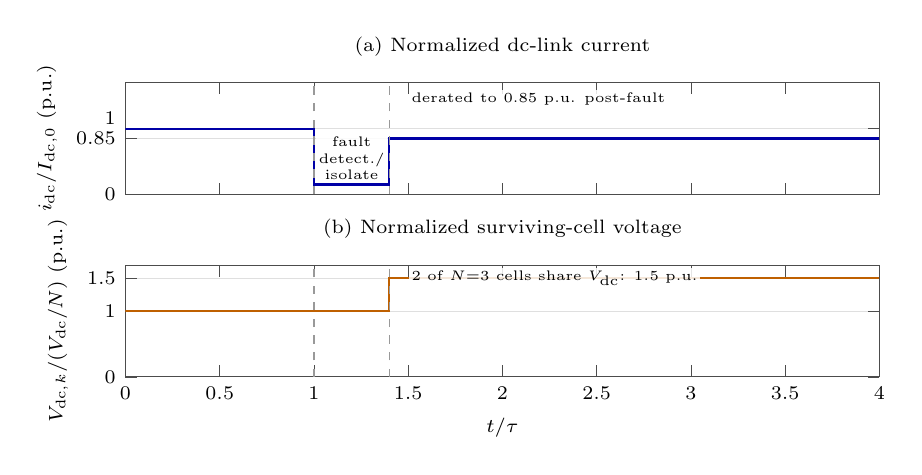
\begin{tikzpicture}
\begin{axis}[
  name=axtop,
  width=0.92\linewidth, height=3.0cm,
  xmin=0,xmax=4, ymin=0,ymax=1.7,
  ylabel={$i_{\mathrm{dc}}/I_{\mathrm{dc},0}$ (p.u.)},
  title={(a) Normalized dc-link current},
  title style={font=\scriptsize}, label style={font=\scriptsize},
  tick label style={font=\scriptsize},
  ymajorgrids, grid style={gray!25},
  xticklabels=\empty,
  ytick={0,0.85},
  extra y ticks={1},
  extra y tick labels={1},
  extra y tick style={tick label style={yshift=1.3mm}},
  axis line style={black!70}, tick style={black!70},
]
\addplot[blue!65!black,thick] coordinates
  {(0,1)(1,1)(1,0.15)(1.4,0.15)(1.4,0.85)(4,0.85)};
\node[font=\tiny,anchor=north west,fill=white,fill opacity=0.85,
  text opacity=1,inner sep=1pt] at (axis cs:1.5,1.6)
  {derated to 0.85~p.u. post-fault};
\draw[dashed,black!40,thin] (axis cs:1,0) -- (axis cs:1,1.7);
\draw[dashed,black!40,thin] (axis cs:1.4,0) -- (axis cs:1.4,1.7);
\node[font=\tiny,align=center,fill=white,fill opacity=0.85,
  text opacity=1,inner sep=1pt] at (axis cs:1.2,0.55)
  {fault\\detect./\\isolate};
\end{axis}
\begin{axis}[
  at={(axtop.south west)}, anchor=north west, yshift=-9mm,
  width=0.92\linewidth, height=3.0cm,
  xmin=0,xmax=4, ymin=0,ymax=1.7,
  xlabel={$t/\tau$}, ylabel={$V_{\mathrm{dc},k}/(V_{\mathrm{dc}}/N)$ (p.u.)},
  title={(b) Normalized surviving-cell voltage},
  title style={font=\scriptsize}, label style={font=\scriptsize},
  tick label style={font=\scriptsize},
  ymajorgrids, grid style={gray!25},
  ytick={0,1,1.5},
  axis line style={black!70}, tick style={black!70},
]
\addplot[orange!75!black,thick] coordinates
  {(0,1)(1.4,1)(1.4,1.5)(4,1.5)};
\node[font=\tiny,anchor=north west,fill=white,fill opacity=0.85,
  text opacity=1,inner sep=1pt] at (axis cs:1.5,1.66)
  {2 of $N{=}3$ cells share $V_{\mathrm{dc}}$: $1.5$~p.u.};
\draw[dashed,black!40,thin] (axis cs:1,0) -- (axis cs:1,1.7);
\draw[dashed,black!40,thin] (axis cs:1.4,0) -- (axis cs:1.4,1.7);
\end{axis}
\end{tikzpicture}
\caption{Illustrative, analytically derived example of the post-fault
current derating and remaining-cell voltage step-up for a
representative $N=3\to2$ case (one of three cells isolated after a
fault); this is not measured or simulated data. (a) Normalized
dc-link current, derated post-fault per
\eqref{eq:fault_power_redistribution}. (b) Normalized remaining-cell
voltage, stepping from 1~p.u. to $N/(N-1)=1.5$~p.u.
\eqref{eq:spb_voltage_sum} once two cells must share $V_{\mathrm{dc}}$.
Both panels share the same time axis.}
\label{fig:spb_fault_response}
\end{figure}

Reliability remains ambiguous because increasing cell count provides
more potential degraded states but also more components that can
fail. System or mission reliability is therefore
more meaningful than component count alone. Markov-chain analysis has
been applied to related fault-tolerant IMMDs to distinguish healthy,
degraded, and failed states \cite{Swanke2022MarkovReliability}, while
integrated distributed traction drives provide additional evidence that
fault tolerance must include both the machine and the local converter
architecture \cite{Hennen2012DistributedIMMD,Wolmarans2008IntegratedFT}.

The direct SPB literature therefore demonstrates the feasibility of
post-fault operation and online reconfiguration, but not yet
automotive-level fault coverage. Detection and isolation time,
short-circuit energy, capacitor and sensor faults, communication loss,
post-fault thermal loading, diagnostic coverage, and deterministic
functional-safety transitions remain important validation topics.

% ============================================================================
\section{Research Gaps and Future Directions}
\label{sec:future_directions}
% ============================================================================

SPB operation, modulation, balancing, and modular control are
established, but the evidence needed for automotive architecture
selection remains incomplete. The key gaps are not additional
proof-of-concept control schemes but high-power validation and
system-level comparisons under common boundary conditions.

\subsection{High-Power Validation and Standardized Benchmarking}

Building on the laboratory-scale validation status noted in
Section~\ref{sec:evolution}, future
prototypes should target several-hundred-kilowatt scale
with realistic dc voltage, thermal, switching-overshoot, and EMI
constraints, among others,
benchmarked directly against a two- or three-level reference drive under
the same machine requirements, semiconductor generation, cooling
boundary, and mission. The scale of benefit that motivates this effort
is not merely hypothetical: a segmented, interleaved traction-drive
system operating at 55~kW has reported a 55--89\% reduction in dc-bus
capacitor ripple current relative to a conventional single-bridge
drive \cite{Su2012SegmentedTraction}, an order of magnitude above the
power level of most direct SPB studies and a useful automotive-scale
reference point for the interleaving benefit discussed in
Section~\ref{sec:modulation}.

Standardized reporting is also needed: published studies vary in power
level, cooling, filtering, and semiconductor generation, and
comparisons can shift materially with the chosen switching-energy
interpolation, temperature correction, and current-derating
assumptions. Reference operating points, efficiency maps, measured
parasitics, and open device/loss-model data would improve
reproducibility as semiconductor technology evolves.

A practical development path should also separate the questions that
can be answered at different hardware scales; Table~\ref{tab:validation_ladder}
proposes a validation ladder so that a low-power proof of one control
function is not read as evidence of automotive readiness.

\begin{table}[!t]
\centering
\caption{Suggested Validation Ladder for Automotive SPB Research}
\label{tab:validation_ladder}
\renewcommand{\arraystretch}{1.05}
\setlength{\tabcolsep}{3pt}
\begin{tabular}{p{1.55cm}p{2.55cm}p{3.35cm}}
\hline
\textbf{Stage} & \textbf{Primary purpose} & \textbf{Minimum evidence}\\
\hline
Cell / double-pulse & Device and commutation feasibility & Overshoot, switching energy, thermal impedance, protection\\
Multi-cell bench & Balancing and modulation & Cell-voltage spread, ripple, timing mismatch, transient stability\\
Dynamometer & Converter--machine interaction & Torque--speed map, efficiency, harmonics, CM/EMI, thermal limits\\
Mission / vehicle-relevant & Architecture value & Drive-cycle energy, cooling, fault derating, reliability and packaging\\
\hline
\end{tabular}
\end{table}

A community benchmark defining one passenger-car and one heavy-duty
traction case -- common dc-voltage range, power, torque--speed
envelope, coolant temperature, modulation limits, and EMC boundary,
with a VECTO-derived mission for heavy-duty work -- would let competing
architectures be compared under comparable electrical and thermal duty
without forcing a single reference machine. Reporting should extend the
same way: beyond peak efficiency, prototypes should state cell-voltage
spread, capacitor ripple current, common-mode current, and post-fault
capability, among other operating-point metrics, linking the
modulation, balancing, semiconductor, and reliability literatures into
transferable evidence.

\subsection{Cell Count, Reliability, and Cost Co-Design}

The optimum cell count $N$ remains the central unresolved design
question: as established in Section~\ref{sec:operating_principle},
the voltage-versus-component-count tradeoff shifts the optimum as
SiC, GaN, packaging, and cooling evolve
\cite{WBGTractionReview2025,Post800V2026}. A
common-platform comparison of a few-cell 650-V GaN SPB against a
many-cell low-voltage GaN SPB, using real commercial devices, would be
valuable; the GaN comparison in \cite{Rohner2024GaN} is a useful
starting point but should be extended to automotive power with current
parallelization, machine voltage/speed constraints, dc-link
capacitance, cooling, and mission energy.

Converter, machine, and thermal models, among others, should
be co-optimized rather than designed sequentially. Existing phase-count
studies show machine design changes with SPB cell number
\cite{Bringezu2020SPB}; the missing step is a complete automotive
co-design using vehicle-level energy, volume, mass, cost, and
reliability as a joint objective.

Reliability is part of that objective: future studies should combine
semiconductor, capacitor, sensor, gate-driver, communication, and
winding faults (Section~\ref{sec:fault_reconfiguration};
\cite{Nikouie2016Fault,Verkroost2024Reconfiguration}) in one
state-based, Markov-style framework as used for related fault-tolerant
IMMDs \cite{Swanke2022MarkovReliability}, keeping \emph{component
failure}, \emph{module isolation}, and \emph{loss of vehicle function}
distinct.
An $N$-cell drive may survive with $N-1$ active modules, but its
torque--speed envelope, module thermal loading, and dc-voltage margin
all change, so reliability data should pair with a post-fault
capability model -- not a series reliability block diagram -- to
compare availability, limp-home power, and mission completion
probability against efficiency.

Cost and sustainability assessment should use the same $N$-dependent
framing: increasing $N$ can reduce per-switch die cost but tends to
increase isolated gate supplies, sensing channels, and assembly
operations, among others, almost linearly, while a
repeated converter--winding module can gain from common tooling and
automated assembly -- a balance likely to differ between high-volume
passenger vehicles and lower-volume heavy-duty systems. The same
accounting should separate production, operation, maintenance, and
end-of-life impact over one vehicle mission and service life, since
modular repair and longer service life can offset the added production
impact of extra components.

Overall, SPB research must move from demonstrating that the
architecture operates toward demonstrating where it is better: whether
it gives a measurable vehicle-level advantage over mature two- and
three-level architectures once machine design, thermal management,
EMC, reliability, manufacturing, and cost are included.

% ============================================================================
\section{Conclusion}
\label{sec:conclusion}
% ============================================================================

This paper reviewed stacked polyphase bridge (SPB) converters --
series-stacked two-level bridges each feeding an electrically
separated winding group -- as a candidate architecture for future
high-voltage traction drives, partitioning the dc-link voltage while
introducing converter--machine modularity, distributed control, and
fault-management opportunities.

The review also shows that the semiconductor voltage advantage cannot
be separated from the complete traction system. Increasing cell count
adds converter, control, and insulation overhead, so SPB does not
eliminate the complexity of high-voltage conversion but redistributes
it between semiconductor technology, machine architecture, and
control. WBG development makes this trade increasingly relevant,
particularly where SPB can move a high-voltage traction system toward
lower-voltage GaN devices; whether that approach is advantageous
depends on whether the device-level gains compensate for the
additional modular hardware and machine requirements.

The remaining step is application-level validation at representative
power, dc voltage, thermal conditions, EMI constraints, and vehicle
missions. SPB should ultimately be judged not as another multilevel
converter, but as a modular traction-drive architecture that exchanges
semiconductor blocking-voltage stress for converter--machine
modularity. Its competitiveness depends on whether that exchange
produces a measurable vehicle-level benefit.


\section*{Acknowledgment}
The authors used Claude (Anthropic) for language editing, structural
organization, and drafting assistance during manuscript preparation.
All technical claims, calculations, references, interpretations, and
final editorial decisions were reviewed and approved by the authors.

\bibliographystyle{jabbrv_IEEEtran}
\bibliography{ref}

\end{document}
